\documentclass[UTF8]{ctexart}
\usepackage{geometry}
\usepackage{amsmath}
\usepackage{amsfonts}
\usepackage{lmodern}
\usepackage{graphicx} %插入图片的宏包
\usepackage{float} %设置图片浮动位置的宏包
\geometry{a4paper,scale=0.8}
\sectionfont{\bfseries\Large\raggedright}

\title{deep-learning笔记}
\author{徐世桐}
\date{}
\begin{document}
\maketitle

% --------------------------------------------------------------------------
% |                                基本定义                                  |
% --------------------------------------------------------------------------
\section{基本定义}

\noindent \textbf{label标签}:输出结果,$\hat{y} $为计算得到的结果,$y$为实际测量结果\\
\textbf{feature特征}:用于预测标签的输入变量,$x^{(i)}_j$为第i组sample第j号特征\\
\textbf{sample样本}:一组特征的取值和对应的标签输出\\
\textbf{batch}:batch size个sample被分为一组,进行向量化的计算,称$B$\\
\textbf{hyperparameter超参数}:人为设定的参数。如样本个数(批量大小batch size)$|B|$,学习率$\eta $。少数情况下通过学习得到\\
\textbf{W 一层layer的权重矩阵}:行数 = 前层节点数,列数 = 当前层节点数\\
\textbf{全连接层fully-connected layer/稠密层dense layer}:此层所有节点都分别和前一层所有节点连接\\
\textbf{sigmoid函数}:$\sigma(x) = \frac{1}{1+e^{-x}}$\\
\textbf{tanh函数}:$tanh(z) = \frac{e^z - e^{-z}}{e^z + e^{-z}}$\\
\textbf{softmax函数}:$softmax(Y) = \frac{exp(y)}{\sum_{y' \in Y} exp(y') } $,将数值输出转化为概率值,1. 值为正\ 2. 值总和为1\\
\textbf{Parapetric ReLU}:

  \begin{equation*}
    PReLU(x) = \begin{cases}
      \alpha x & x < 0\\
      x & x \geq 0
    \end{cases}
  \end{equation*}
  
  $\alpha$ 训练时更新\\
\textbf{leaky ReLU}:

  同PReLU,$\alpha$为超参数\\
\textbf{Exponential LU}

  \begin{equation*}
    ELU(x) = \begin{cases}
      \alpha (e^x - 1) & x < 0\\
      x & x \geq 0
    \end{cases}
  \end{equation*}\\
\textbf{catagorical cross entropy交叉熵}

  定义:分部p\ 和\ 分部q\ 间的\ cross entropy $H(p, q) = -E_p(\log (q))$。为\ expected value of $log (q)$ with respect to distribution p

  公式:对一样本的输出$\hat{y}^{(i)}$, $H(y^{(i)}, \hat{y}^{(i)}) = -\frac{1}{n}\sum_{j < n}y^{(i)}_jlog(\hat{y}^{(i)}_j)$

  \quad n为输出标签数

  \quad 对一批量的输出使用cross entropy:对每一样本i的$H(y^{(i)}, \hat{y}^{(i)})$求和

  使用:联系两个值概率分部间的差异,即可将数值输出$\hat{y}$和分类结果$y$直接做对比

  \quad \textbf{适用于multi-class classification,仅有唯一类别作为输出}

  \quad \quad 原因:catagorical cross entropy假设\ 其余类别输出\ 随\ 期望类别输出升高\ 而降低,则忽略其余类别的输出是否为0

  \quad 仍可和softmax同时使用,softmax将可能性先转换为正数并和为1,随后使用cross entropy\\
\textbf{binary cross entropy}

  公式:$H(y, \hat{y}) = -y \space log(\hat{y}) + (1 - y)log(1 - \hat{y})$

  \quad $\hat{y}, y$为单一标量
  
  使用:
  
  \quad \textbf{使用于单个输出的logistic regression,或multi-label regression}

  \quad \quad multi label时将每一label分别进行binary cross entropy后求和
  
  \quad multi-label regression代价值为每一label预测值的binary cross entropy求和\\
\textbf{指数加权移动平均}

  $y_t = \gamma y_{t-1}+(1-\gamma)x_t$\\
\textbf{小批量乘法}

  对$n$个形状为$(a, b)$矩阵$X_1, X_2, ..., X_n$,$n$个形状为$(b, c)$矩阵$Y_1, Y_2, ..., Y_n$,小批量乘法结果为$X_1Y_1, X_2Y_2, ..., X_nY_n$

  * 特指被word2vec使用的乘法,其他模型仍根据矩阵乘法,非所有批量乘法都使用\ 小批量乘法\\
\textbf{Sigmoid二元交叉熵损失函数}

  得到向量$P = [p_1, ..., p_n]$,向量$L = [l_1, ..., l_n]$,掩码向量$M = [m_1, ..., m_n]$

  \quad $p_i$标记$i$位置事件的可能性,$l_i$标记期望$i$位置的事件发生$(l_i = 1)$或不发生$(l_i = 0)$

  计算:

  \quad 1.遍历$L$,若$l_i = 0$,$p'_i = -p_i$

  \quad 2.对$P'$中每一$p'_i$取sigmoid值,对所有$m_i = 1$的$p'_i$求平均值

  整体计算为:$f(P, L, M) = \frac{\sigma(P) \odot (-1)^L \odot M}{sum(M)}$\\
\textbf{Laplace smoothing}

  令n(x)为x的出现个数,m为词的个数,n为所有词出现次数总和
  
  \quad 目标:解决在特殊词组$[x, x']$出现次数过小时$n(x, x')$较小。导致原公式$P(x' | x) = \frac{n(x, x')}{n(x)}$值过小
    
  $P(x) = \frac{n(x) + \epsilon_1 / m}{n + \epsilon_1}$

  $P(x' | x) = \frac{n(x, x') + \epsilon_2 P(x')}{n(x) + \epsilon_2}$

  $P(x'' | x, x') = \frac{n(x, x', x'') + \epsilon_3 P(x' | x)}{n(x, x') + \epsilon_3}$\\
\textbf{Laplace operator $\Delta$}

  对函数$f(x, y)$:$\Delta f = \frac{d^2f}{dx^2} + \frac{d^2f}{dy^2}$\\
\textbf{函数卷积}

  对函数$f, g : \mathbb{R}^n \mapsto \mathbb{C}$,定义函数卷积$(f * g)(x) = \int_{\mathbb{R}^n} f(\tau)g(x - \tau) \,d\tau$

  \quad $f, g$取离散值时,$(f * g)(x) = \sum_\tau f(\tau)g(x - \tau)$

  \quad $f(m), g(m)$都为标量。$f(x)g(x - \tau)$意为\textbf{将卷积核左移n后和$f(x)$按元素相乘求和}

  交换律:$f * (g * h) = (f * g) * h$
  
  结合律:$f * (g + h) = (f * g) + (f * h)$

  求导:$\frac{d }{dx}(f * g) = \frac{d f}{dx} * g = f * \frac{dg}{dx}$
  
  性质:

  \quad Commutativity:$f * g = g * f$
  
  \quad Associativity:$f * (g * h) = (f * g) * h$,$a(f * g) = (af) * g$
  
  \quad Distributivity:$f * (g + h) = (f * g) + (f * h)$\\
\textbf{shift invarient}

  对于一操作$f$,$f(x) = f(x + \epsilon)$称shift invarient。即当输入图片目标移动\ 仍能输出正确分类
  
  如:全连接层,最大池化层。不论目标位置,输出标签/张量值相同\\
\textbf{shift equivalent}

  输出应随输入目标移动而移动

  如:卷积层。目标移动后输出矩阵值改变\\
\textbf{Cosine distance}

  $d(x, y) = \frac{x \cdot y}{\|x\|\|y\|}$

  即向量x,y夹角\\
\textbf{Euler-Lagrange equation}

  定义:$u$为一函数,$u'(t) = \frac{du(t)}{du}$,$S(u)= \int_{t} L(t, u(t), u'(t)) \,dt$。

  Theorem:u为一S的stationary point
  
  \quad iff $\frac{L(t, u(t), u'(t))}{du} - \frac{L(t, u(t), u'(t))}{d(u'(t))dt}$

% --------------------------------------------------------------------------
% |                           perceptron 分类算法                           |
% --------------------------------------------------------------------------
\section{perceptron 分类算法}
\noindent \textbf{前向传播}

  $\hat{y} = h(W^Tx + b)$
  
  激活函数h(x)

  \quad 当$x > 0$时$h(x) = 1$

  \quad 当$x \leq 0$时$h(x) = 0$\\
\textbf{迭代}

  $\theta_i = \theta_i + \alpha(y - h(x))x_i$
  
  \quad $\alpha$为学习率

% --------------------------------------------------------------------------
% |                            反向传播公式推导                              |
% --------------------------------------------------------------------------
\section{反向传播公式推导}
\noindent \textbf{向量求导定义}

  标量对向量求导:$\frac{ds}{d\textbf{v}} = \begin{bmatrix}
    \frac{ds}{dv_0} & \frac{ds}{dv_1} & ... & \frac{ds}{dv_n}
    \end{bmatrix}$

  向量对向量求导:$\frac{d\textbf{u}}{d\textbf{v}} = \begin{bmatrix}
    \frac{du_0}{dv_0} & ... & \frac{du_0}{dv_n} \\
    ... & ... & ... \\
    \frac{du_m}{dv_0} & ... & \frac{du_m}{dv_n}
    \end{bmatrix}$
  
  对$z = Wx$有:
  
  \quad $\frac{z}{x} = W$
  
  \quad $\frac{dL}{dW} = \frac{dL}{dz}x$

  对$z = xW$有:
  
  \quad $\frac{dz}{dx} = W^T$

  \quad $\frac{dL}{dW} = x^T\frac{dL}{dz}$\\
\textbf{对一层前向传播$g(Z)$, $Z = XW + \vec{b}$}

  X为前一层输入,即前一层g(X)矩阵
  
  g此处为广播操作,对矩阵Z中每一元素求activation 值
  
  +此处为广播操作,对每行XW加偏差\\
\textbf{求权重斜率}
  
  单一权重值求导:$\frac{dL}{dw_{ij}} = \sum_k \frac{dL}{dZ_{kj}} X_{ki}$

  对权重矩阵求导:$\frac{dJ}{dW} = X^T\frac{dL}{Z}$\\
\textbf{对前一层输出X求导}

  $\frac{dL}{dX_{ij}} = \sum_k W_{jk}\frac{dL}{dZ_{ik}}$

  $\frac{dL}{dX} = \frac{dL}{dZ}W^T$\\
\textbf{对偏差求导}

  $\frac{dL}{db_i} = \sum_k \frac{dL}{dZ_{ki}}$

  $\frac{dL}{d\vec{b}} = \vec{1}^T\frac{dL}{dZ}$\\
\textbf{激活函数求导}

  反向传播:$\frac{dL}{dx} = \frac{dL}{dg(x)} \cdot g'(x)$
  
  \quad $g', \cdot$ 为按元素操作

  sigmoid $g(z) = \frac{1}{1 + e^{-z}}$ 求导: $g'(z) = g(z)(1 - g(z))$

  tanh $g(z) = \frac{e^z - e^{-z}}{e^z + e^{-z}}$ 求导: $g'(z) = 1 - g(z)^2$

  softmax $\hat{y}_i = softmax(z_i)$ $J = -\frac{1}{N}\sum_{i=1}^{N}\sum_{c=1}^{C}y_{ic}log(\hat{y}_{ic})$,
  
  \quad 求导: $\frac{dL}{dz} = \frac{1}{N}(\hat{y} - y)$\\
\textbf{验证gradient计算}

  1.得到斜率$\frac{dL}{dW}$

  2.微调$W + \epsilon$,计算$L(W)$,$\frac{dL}{dW} \approx \frac{L(W + \epsilon) - L(W - \epsilon)}{2\epsilon}$

  3.比较两$\frac{dL}{dW}$值是否相近

% --------------------------------------------------------------------------
% |                       linear regression线性回归                         |
% --------------------------------------------------------------------------
\section{linear regression线性回归}
\noindent \textbf{平方代价函数}:$J(\theta ) = \frac{1}{|B|} \sum_{i = 1}^{|B|} J^{(i)}(\theta ) = \frac{1}{2|B|} \sum_{i = 1}^{|B|} (\hat{y}^{(i)} - y^{(i)})^2  $,为所有样本误差的平均值\\
\textbf{迭代}:$\theta_i = \theta_i - \frac{\eta}{|B|}\sum_{j\in B} \frac{d J^{(j)}(\theta)}{d \theta_i}$,即对所有sample训练一次,得到label差值,对每一参数减\ 斜率*学习率\ 的平均值
  
  当使用平方代价函数:
  
  \quad $\theta_i = \theta_i - \frac{\eta}{|B|}\sum_{i\in B} x^{(j)}_i(x^{(j)}_1\theta_1 + x^{(j)}_2\theta_2 + ... + const - y^{(j)}) = \theta_i - \frac{\eta}{|B|}\sum_{i\in B}x^{(i)}(\hat{y}^{(j)} - y^{(j)})$

  \quad $const = const - \frac{\eta}{|B|}\sum_{i\in B} (x^{(j)}_1\theta_1 + x^{(j)}_2\theta_2 + ... + const - y^{(i)}) = const - \frac{\eta}{|B|}\sum_{i\in B}(\hat{y}^{(j)} - y^{(j)})$

  \quad 对样本i的偏导数向量为$\nabla _{\theta}J^{(i)}(\theta) = 
    \begin{bmatrix}
    x^{(i)}_1 \\
    x^{(i)}_2 \\
    ... \\
    1
    \end{bmatrix}(\hat{y}^{(i)} - y^{(i)})
    $\\
\textbf{交叉熵代价函数}:$J(\theta) = \frac{1}{|B|}\sum_{i\in B} H(y^{(i)}, \hat{y}^{(i)})$\\
\textbf{softmax线性回归}:单层神经网络,使用softmax函数得到分类,使用cross entropy计算代价\\
\textbf{过拟合问题}

  \textbf{1.权重衰减regularisation}:在代价函数中惩罚高权重的值,尽可能使所有权重值减小

  \quad \textbf{每一权重的正则化值都会影响其余所有权重的斜率},由于正则化项为标量加入代价函数

  \quad L2 正则化代价函数 = $J(\theta) + \frac{\lambda}{2}\sum_{w\in W}w^2$,即 $J(\theta) + \frac{\lambda}{2} * $ 所有权重的平方和。$\lambda$为超参数,决定权重衰减的程度

  \quad \quad 求导 = $\frac{dL}{dw} + \lambda w$
  
  \quad L1 正则化代价函数 = $J(\theta) + \lambda \sum_{w\in W} |w|$,即 $J(\theta) + \frac{\lambda}{2} * $ 所有权重绝对值和。

  \quad \quad 求导 = $\frac{dL}{dw} + \lambda sign(w)$

  \textbf{2.丢弃法dropout}

  \quad 每一权重(不包括const)有p的几率 $\theta' = 0$,有1-p的几率 $\theta' = \frac{\theta}{1-p}$

  \quad \quad 常用p = 0.5

  \quad \quad \textbf{仅将输出值部分设为0,不删除原权重}

  \quad \quad \textbf{反向传播时被隐藏的神经元向上一层传斜率为0}

  \quad 为了得到确切的值,在测试模型时较少使用
  
  \quad \quad \textbf{取消dropout层后需将输出按元素全部乘p值,否则测试时输出参数值为训练时$\frac{1}{p}$倍}\\
\textbf{初始化参数}

  \textbf{1.MXNet默认随机初始化}:所有权重$\sim N(0, 1)$的normal distribution,所有const取0

  \textbf{2.Xavier随机初始化}:对一全连接层,输入个数a,输出个数b,则所有参数$\sim U(-\sqrt{\frac{6}{a+b}}, \sqrt{\frac{6}{a+b}})$\\
\textbf{预处理数据集}

  \textbf{1.特征标准化 standardization/z-normalization}:$x' = \frac{x - \mu}{\sigma}$,即统计中z值

  \textbf{2.离散值转换成指示特征}:对于一个可取值为A, B, C的离散输入值,转换成3个数值输入。即如果原输入为A,转换后3个数值输入为1,0,0。原离散值为B则转换后为0,1,0
  
  \textbf{3.Min-max normalisation}:将每一特征值拉伸为[a, b],取一特征的最值$X_{min}, X_{max}$,则拉伸后每一特征值$X' = a + \frac{(X - X_{min})(b - a)}{X_{max} - X_{min}}$
  
  \quad 存储a, b, $X_{min}$, $X_{max}$值可将数据逆操作 得到原数据集\\
\textbf{结构}
  
  - 将训练集分组,每组batch\_size个sample。
  
  - 对这个batch的数据进行向量化计算,计算loss,\textbf{斜率清零},计算斜率,调用优化函数。

  - 即每一batch使用相同的权重\ 偏差。一次训练一共历多次所有sample,一次遍历进行$\frac{sample\_size}{|B|}$次向量化计算\\
\textbf{隐藏层必定使用激活函数,输出层可选使用激活函数}\\
% \textbf{梯度下降的过程中一直使用真实梯度,无需减小学习率}?\\
\textbf{全连接神经网络常用神经元数同输入特征个数,每层神经元个数相同}


% --------------------------------------------------------------------------
% |                convolutional neural network卷积神经网络                  |
% --------------------------------------------------------------------------

\section{convolutional neural network卷积神经网络}
\noindent \textbf{互相关运算}:

  输入一个二维数组,和\textbf{二维核kernel}进行互相关运算,得到二维数组

  \textbf{二维核/卷积核/filter 过滤器}:在输入数组上滑动,每次和二维数组矩阵一部分按元素相乘 求和,作为输出矩阵的元素\\
\textbf{二维卷积层}:

  将输入和卷积核做互相关运算,结果加上const作为输出\\
\textbf{特征图}:输出矩阵可看做是输入矩阵的表征,称特征图\\
\textbf{感受野receptive field}:
  
  对输出矩阵一元素x,所有可能影响其值的输入矩阵元素称感受野

  感受野可能大于实际输入的矩阵边界\\
\textbf{填充padding}:
  
  在输入矩阵外侧添加全零元素,使得输出矩阵的维度增加,由于可用的感受野增加。

  常使用奇数kernel,添加$\lfloor \frac{kernel}{2}\rfloor $的填充,使得输出矩阵和输入矩阵纬度一样\\
\textbf{步幅stride}:

  定义每次感受野向左/向下移动的纬度\\
\textbf{dilation}

  在较大卷积核中仅选择某些矩阵元素赋权重进行卷积计算,其余权重为0\\
\textbf{多通道输入输出}:

  当输入的数据包含多个矩阵,即多通道输入,例:RGB图像有3个输入通道

  对$c_i$输入, $c_o$输出的卷积层,kernel shape为($c_o$, $c_i$, 行数,列数)

  \quad 每一输入通道有唯一的kernel ($c_i$, 行数,列数)对应,进行互相关运算后结果矩阵相加,作为一条输出通道的结果

  \quad 多组($c_i$, 行数,列数)分别产生输出通道的结果矩阵,则有$c_o$条输出通道\\
\textbf{池化层}:
  
  作用:1 为了防止当输入变化时,输出立即随之更改。2\ 减少计算量

  池化窗口,同卷积层的感受野。限定某块输入被同时考虑,同样有stride,可对输入padding

  \quad 1. 最大池化层:取池化窗口内最大的输入

  \quad 2. 平均池化层:取池化窗口平均值

  \textbf{多输入通道间池化结果不相加,即\ 输入通道数 = 输出通道数}\\
\textbf{LeNet卷积神经网络}

  \textbf{1.使用2组\ 卷积计算层\ 激活函数层\ 池化层}

  \quad 输出通道数分别为6,16。卷积层\ kernel 为(5, 5), 步幅为1, 无padding

  \quad 激活函数层\ 对每一元素做sigmoid

  \quad 最大池化层\ 窗口(2, 2),步幅为2

  \textbf{2.使用3组全连接层}

  \quad 节点数120, 84, 输出节点数。除输出层使用sigmoid激活函数,即120 84节点层

  \quad 将(批量大小, 通道数, height, width) 看做 (批量大小,通道数 * height * width)处理\\
\textbf{AlexNet深度卷积神经网络}:

  除输出层和丢弃层,全部使用relu做激活函数

  \textbf{卷积部分}
  
  \quad - 2组\ 卷积层 + 最大池化层
  
  \quad \texttt{nn.Conv2D(96, kernel\_size=11, strides=4, activation='relu')}

  \quad \texttt{nn.MaxPool2D(pool\_size=3, strides=2)}

  \quad \texttt{nn.Conv2D(256, kernel\_size=5, padding=2, activation='relu')}

  \quad \texttt{nn.MaxPool2D(pool\_size=3, strides=2)}
  
  \quad - 3卷积层 + 1最大池化层,高输出通道,低卷积窗口
  
  \quad \texttt{nn.Conv2D(384, kernel\_size=3, padding=1, activation='relu')}
  
  \quad \texttt{nn.Conv2D(384, kernel\_size=3, padding=1, activation='relu')} 
  
  \quad \texttt{nn.Conv2D(256, kernel\_size=3, padding=1, activation='relu')}
  
  \quad \texttt{nn.MaxPool2D(pool\_size=3, strides=2)}

  \textbf{全连接层部分}
  
  \quad - 两hidden layer全连接层\ 使用丢弃法

  \quad \texttt{nn.Dense(4096, activation="relu"), nn.Dropout(0.5)}
  
  \quad \texttt{nn.Dense(4096, activation="relu"), nn.Dropout(0.5)}
  
  \quad \texttt{nn.Dense(10)} //\ 根据需求改变输出层节点,原论文为1000\\
\textbf{VGG使用重复元素网络}

  \textbf{VGG基础块}

  \quad 数个(3, 3)kernel 1填充卷积层 + 1个(2, 2)窗口\ 2步幅最大池化层

  \quad 卷积层\ 层数\ 通道数为超参数,一VGG块中每一卷积层有相同通道数

  VGG 神经网络由\ 数个VGG块 + 数个全连接层\ 组成

  例:\textbf{VGG-11}
  
  \quad 1.\ (1, 64) (1, 128) (2, 256) (2, 512) (2, 512) 5层VGG块

  \quad \quad (n, m) 代表此VGG块使用n层卷积层,各有m通道
  
  \quad 2.\ 3层全连接层,实现同AlexNet的全连接层部分
  
  \quad 共8层卷积层+3层全连接层,所以称VGG-11\\
\textbf{NiN神经网络}

  \textbf{NiN块}

  \quad 1个自定义卷积层 + 2层 (1, 1)kernel 卷积层,3层卷积层都不包含池化层

  \quad 自定义卷积层可设置kernel,步幅,填充。
  
  \quad (1, 1)卷积层可设置通道数 (=自定义层通道数),其余固定为默认值

  NiN神经网络有多组\ (NiN块 + 池化层)
  
  例:\textbf{NiN模型}

  \quad - NiN块部分

  \quad \texttt{nin\_block(96, kernel\_size=11, strides=4, padding=0)}

  \quad \texttt{nn.MaxPool2D(pool\_size=3, strides=2)}

  \quad \texttt{nin\_block(256, kernel\_size=5, strides=1, padding=2)}

  \quad \texttt{nn.MaxPool2D(pool\_size=3, strides=2)}

  \quad \texttt{nin\_block(384, kernel\_size=3, strides=1, padding=1)}

  \quad \texttt{nn.MaxPool2D(pool\_size=3, strides=2)}

  \quad - 在NiN块部分结束后加入丢弃层

  \quad \texttt{nn.Dropout(0.5)}

  \quad - 转化为对应分类个数的输出

  \quad \texttt{nin\_block(10, kernel\_size=3, strides=1, padding=1)}

  \quad \texttt{nn.GlobalAvgPool2D()} // 全局平均池化层,每一通道取矩阵所有元素的平均值

  \quad \texttt{nn.Flatten()} // 平均池化层结果即分类结果,flatten仅用于改变shape\\
\textbf{GoogLeNet含并行结构神经网络}

  \textbf{Inception块}
  \begin{figure}[H] %H为当前位置,!htb为忽略美学标准,htbp为浮动图形
    \centering %图片居中
    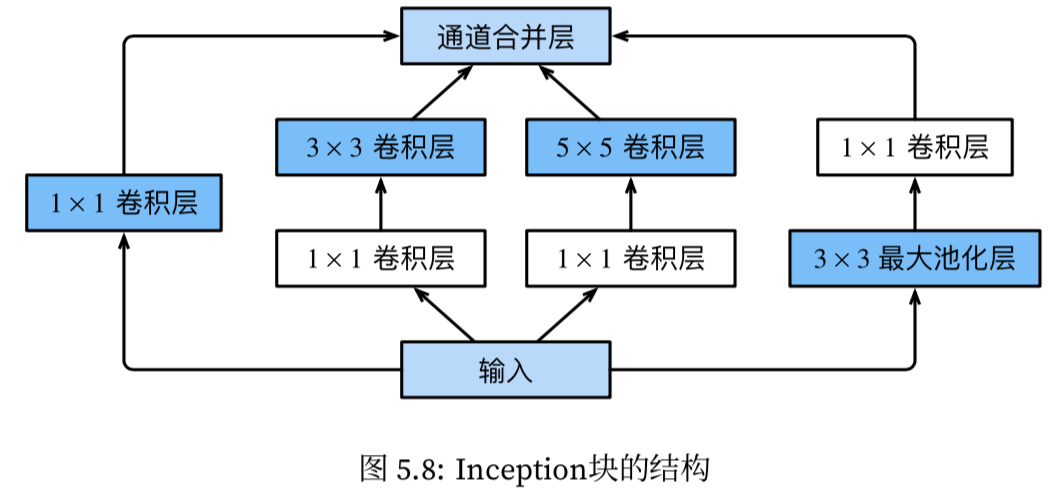
\includegraphics[width=0.6\textwidth]{note_images/inception_block.png} %插入图片,[]中设置图片大小,{}中是图片文件名
  \end{figure}

  \quad inception块结构表示:($n_1$, ($n_{21}$, $n_{22}$), ($n_{31}$, $n_{32}$), $n_4$) 
  
  \quad \quad 第一线路使用$n_1$通道
 
  \quad \quad 第二线路第一卷积层使用$n_{21}$通道,第二层卷积层使用$n_{22}$通道 1填充
 
  \quad \quad 第三线路第一卷积层使用$n_{31}$通道,第二层卷积层使用$n_{32}$通道 2填充
  
  \quad \quad 第四线路第一最大池化层使用(3, 3)窗口 1填充,第二层卷积层使用$n_4$通道

  \quad 每一卷积层都使用relu激活函数

  \quad 所有层输出作为不同通道结果,即最终有$n_1 + n_{22} + n_{32} + n_4$通道

  GoogLeNet结构:

  \quad 5个串联模块,每一卷积层使用relu激活函数,每一模块间使用 (3, 3)窗口\ 步幅2\ 1填充\ 池化层

  \quad 1. 64通道(7, 7)kernel 2步幅\ 3填充卷积层 + 模块间池化层

  \quad 2. 64通道(1, 1)kernel卷积层 + 64 * 3通道(3, 3)kernel 1填充卷积层 + 模块间池化层

  \quad 3. 串联2 inception 块 + 模块间池化层,分别有结构

  \quad \quad (64, (96, 128), (16, 32), 32),通道比\texttt{2:4:1:1}

  \quad \quad (128, (128, 192), (32, 96), 64),通道比\texttt{4:6:3:2}

  \quad 4. 串联5 inception 块 + 模块间池化层,

  \quad \quad (192, (96, 208), (16, 48), 64)

  \quad \quad (160, (112, 224), (24, 64), 64)

  \quad \quad (128, (128, 256), (24, 64), 64)

  \quad \quad (112, (144, 288), (32, 64), 64)

  \quad \quad (256, (160, 320), (32, 128), 128)

  \quad 5. 串联2 inception 块 + 全局平均池化层

  \quad \quad (256, (160, 320), (32, 128), 128)

  \quad \quad (384, (192, 384), (48, 128), 128)

  \quad 6. 全连接层,节点数和分类类别数相同

% --------------------------------------------------------------------------
% |                            CNN优化方法                                  |
% --------------------------------------------------------------------------
\section{CNN优化方法}
\noindent \textbf{批量归一化 batch normalization}

  \textbf{1. 对全连接层做批量归一}

  \quad 处于\ 输入的仿射变换\ 和\ 激活函数间,即\ 输出 = $\phi (BN(x))$ $BN$为批量归一计算

  \quad 1. 对于批量仿射 $x = Wu + b$,求标准化$\hat{x}_i = \frac{{x_i} - \mu}{\sqrt{\sigma^2 + \varepsilon }}$。$\mu $和 $\sigma$都为此组仿射变换的结果

  \quad 2. $BN(x) = \gamma * \hat{x}_i + \beta $,$\gamma$拉伸 $\beta$偏移。* + 为按元素加法 乘法

  \textbf{2. 对卷积层做批量归一}

  \quad 处于\ 卷积计算\ 和\ 激活函数\ 间,卷积计算 + 批量归一 + 激活函数 + 池化层

  \quad 各通道独立计算,各有独立拉伸$\gamma$ 偏移$\beta$。
  
  \quad $\sigma$, $\mu$为此通道\ 一批量内\ 所有通道\ 的所有元素\ 的总体方差,平均值

  \quad 得到$\sigma$, $\mu$后对此通道此批量内所有元素求标准化

  \quad 最终对此通道\ 
  \ 偏移\\
\textbf{ResNet残差网络}

  \textbf{残差块}

  \quad 训练时期望输出为f(x) - x,而非直接使用f(x)期望输出。得到f(x) - x后+x得到f(x)

  \quad 1. 卷积层(批量归一) + relu + 卷积层(批量归一) 得到$f(x) - x$
  
  \quad 2. [$f(x) - x$] + [(1, 1)卷积层对(x)卷积结果] + relu激活函数
  
  \quad \quad 第一卷积层:(3, 3)kernel 1填充 (通道数\ 步幅自定义)

  \quad \quad \quad 第234组残差组 第一残差块\ 第一卷积层步幅为2,否则为1

  \quad \quad 第二卷积层:(3, 3)kernel 1填充 1步幅 (通道数自定义)

  \quad \quad +x步骤的(1, 1)卷积层:(通道数\ 步幅自定义) 

  \quad \quad \quad 第234组残差组\ 第一残差块使用(1, 1)卷积层,步幅为2,否则直接+x

  \quad \quad 3层卷积层通道数共享同一自定义值,\textbf{要求2层卷积层输入输出通道数一致}

  ResNet-18模型:共18卷积层

  \quad 1. 64通道(7, 7)kernel 2步幅 3填充\ 批量归一卷积层 + (3, 3)窗口 2步幅 1填充最大池化层

  \quad 2. 4组\ 残差块,每组包含多个残差块

  \quad \quad 第一组 2个残差块\ 输出通道数和1中输出通道数一致
  
  \quad \quad 第二三四组\ 各2个残差块\ 输出通道数为前一层通道数$*2$

  \quad 3. 全局平均池化层 + 对应输出结果数全连接层\\
\textbf{DenseNet稠密连接网络}

  类似ResNet残差网络,+x步变为concat x连在输出结果后,即x直接传向下一层

  \textbf{稠密块}

  \quad 多组(批量归一 + relu + (3, 3)kernel 1填充卷积层 + concat x) 卷积层通道数相同

  \quad concat操作为在通道纬度的concat,即输入x作为额外输出通道。

  \quad 增长率 = 输出通道 - 输入通道 = 卷积层通道数

  \textbf{过渡层}

  \quad 批量归一 + relu + (1, 1)卷积层 + (2, 2)窗口 2步幅平均池化层
  
  \quad 使用(1, 1)卷积层减小通道数,2步幅平均池化层减小矩阵大小

  \quad \quad 卷积层通道数 = 输出通道数 / 2

  DenseNet模型

  \quad 1. 64通道(7, 7)kernel 2步幅 3填充\ 批量归一卷积层 + (3, 3)窗口 2步幅 1填充最大池化层

  \quad 2. 4组稠密块,由3个过渡层分隔

  \quad \quad 4层稠密块卷积层数可以不相同

  \quad 3. 批量归一 + relu + 全局平均池化层 + 对应输出结果数全连接层

% --------------------------------------------------------------------------
% |                             循环神经网络                                 |
% --------------------------------------------------------------------------
\section{RNN循环神经网络}

\noindent 记录数据状态,根据以往状态和当前输入决定输出

  \textbf{仅仅使用前n个词进行预测会将误差叠加,导致产生的输出最终趋向一固定值}\\
\textbf{n阶马尔科夫链}:一个词的出现仅和前n个词有关\\
\textbf{语言模型}:词序($w_1$, $w_2$, ..., $w_T$)的出现可能性为

  $P(w_1, w_2,...,w_T) = \prod_{t=1}^{T} P(w_t|w_{t-(n-1)},...,w_{t-1})$

  称n元语法,每一$w_t$为一时间步中出现的词\\
\textbf{处理语言模型}:将每一文字转化为索引,使用索引做训练参数集\\
\textbf{one\_hot表示}:索引为$i$的词对应one\_hot向量$[v_0 = 0, v_1 = 0, ..., v_i = 1, v_{i+1} = 0, ...]$\\
\textbf{采样方式}:

  $B$ batch size
  
  $T$ 每个样本包含的时间步数

  $S$ 总时间步数

  \textbf{1 随机采样}:

  \quad 在$[0, T)$范围内选择一起始位置$s$,每$T$长度分为一样本。共得到$\lfloor \frac{S - s}{T} \rfloor$样本

  \quad 随机选择$B$个样本作为一批量数据。不同批量间不重复使用样本

  \quad 训练不同样本时不能将前一次隐藏层结果纳入计算
  
  \textbf{2 相邻取样}:

  \quad 同随机采样得到$\lfloor \frac{S - s}{T} \rfloor$样本

  \quad 选择批量中样本时,不同批量的同一位置样本连续。即第2批量0位置的样本为第1批量0位置样本的下一样本

  \quad 仅需在一epoch开始时初始化隐藏层结果,而非在每一批量开始初始化\\
\textbf{裁剪梯度}

  将所有参数斜率拼接成向量$g$,进行裁剪:$g' = min(\frac{\theta}{||g||}, 1)g$
  
  \quad 即所有斜率一次迭代中最多更改$\theta$\\
\textbf{困惑度 perplexity}

  T时间步困惑度$ = exp(-\frac{1}{T}\sum_{i \in T} log(P(n_i | n_1, ..., n_{i-1})))$

  \quad $n_i$为期望的输出词,$P(n_i | n_1, ..., n_{i-1})$即softmax后期望输出词位置的$\hat{y}$

  \quad 即对每一样本,T时长里每一次预测的Softmax Caragorical交叉熵损失值求和,取exp
  
  求多迭代总困惑度:交叉熵按时长T加权求和后取exp值\\
\textbf{强制学习 teaching forcing}:对自然语言人工智能通用

  当预测第$i$时间步$y_i$时使$y_{i-1}$为样本实际上一label,而不是上一次预测的计算结果$\hat{y}_{i-1}$\\
\textbf{RNN实现}

  模型:

  \quad 输入$X_t$,输出$O$:时间步数\ 个\ (批量大小,词典大小)矩阵

  \quad 1.隐藏层$H_t = \phi(X_tW_{xh} + H_{t-1}W_{hh} + b_h)$

  \quad \quad $X_t$为上一时间步的词

  \quad \quad $H_{t-1}$项为隐藏层前一次输出,称隐藏状态,第一个时间步使用全零$H_{t-1}$矩阵

  \quad \quad 简化计算:$X_tW_{xh} + H_{t-1}W_{hh} = [X_t, H_{t-1}][W_{xh}, W_{hh}]^T$

  \quad \quad 激活函数$\phi$为tanh

  \quad 2.输出层$O = HW_{hq} + b_q$
  
  实现:

  \quad 训练时输入一段词序$[w_{0}, w_{l}]$,输出即为预测$[w'_{1}, w'_N]$的词
  
  \quad 批量输入:(批量大小, 时间步数$l$) 每一元素为单个词,即一批量的句子前缀
  
  \quad \quad 输入转换为\ 时间步数\ 个\ (批量大小, 词典大小)矩阵,第$i$矩阵第$j$行对应\ 批量中第$j$样本\ 第$i$时间步的词的one\_hot向量
    
  \quad 计算:预测$T$长度的词序

  \quad \quad 时间步$t$从1开始

  \quad \quad 1.$t = 0$的隐藏状态$H_0$设为全0向量

  \quad \quad 2.$t \leq T$:使用(prefix在t位置的词,隐藏状态$H_{t-1}$)计算\ (t位置预测词,$H_t$)

  \quad \quad \quad \textbf{输出词$[w'_{1}, w'_{T}]$不一定和输入$[w_1, w_T]$一致},但在$[1, T]$时间段内使用输入词$w_{t-1}$,而非上一预测词$w'_{t-1}$\ 进行预测

  \quad \quad \quad 即forced learning。或称warm-up,过程中计算了隐藏状态
  
  \quad \quad 3.$t > T$:使用(上一预测词,$H_{t-1}$)预测

  \quad \quad \quad 训练时标签长度和prefix长度相同,即到达t = T时预测停止
  
  \quad \quad 代价函数对每组\ 预测词和目标词的one\_hot\ 使用softmax交叉熵,求和/求平均
  
  \quad \quad \quad 反向传播仍使用此批量T时长的总代价值,不使用困惑度反向传播\\
\textbf{通过时间反向传播}

  \textbf{有关时间步的损失函数}:$L = \frac{1}{T}\sum_{t = 1}^{T} l(o_t, y_t) $ \textbf{$o_t$此处为单一批量的t时间步输出}

  \textbf{反向传播公式} 
  
  \quad 针对单一样本,假设隐藏层不使用激活函数

  \quad \quad $h_t = W_{xh}x_t + W_{hh}h_{t-1} + b_h$

  \quad \quad $o = W_{hq}h_t$
  
  \quad $\frac{d L}{d o_t} = \frac{1}{T}\frac{d l(o_t, y_t)}{d o_t}$
  
  \quad $\frac{d L}{d W_{qh}} = \sum_{t=1}^{T}\frac{d L}{d o_t}h_t^T$
  
  \quad $\frac{d L}{d h_T} = W_{qh}^T\frac{d L}{d o_T}$
  
  \quad 当t < T:$\frac{d L}{d h_t} = W_{hh}^T\frac{d L}{d h_{t+1}} + W_{qh}^T\frac{d L}{d o_t}$
  
  \quad \quad $ = \sum_{i=t}^{T}(W_{hh}^T)^{T - i}W_{qh}^T\frac{d L}{d o_{T - i + t}}$
  
  \quad $\frac{d L}{d W_{hx}} = \sum_{t=1}^{T}\frac{d L}{d h_t}x^T$
  
  \quad $\frac{d L}{d W_{hh}} = \sum_{t=1}^{T}\frac{d L}{d h_t}h_{t-1}^T$\\
\textbf{GRU 门控循环单元}

  替代原计算隐藏状态方法,应对梯度衰减
  \begin{figure}[H] %H为当前位置,!htb为忽略美学标准,htbp为浮动图形
    \centering %图片居中
    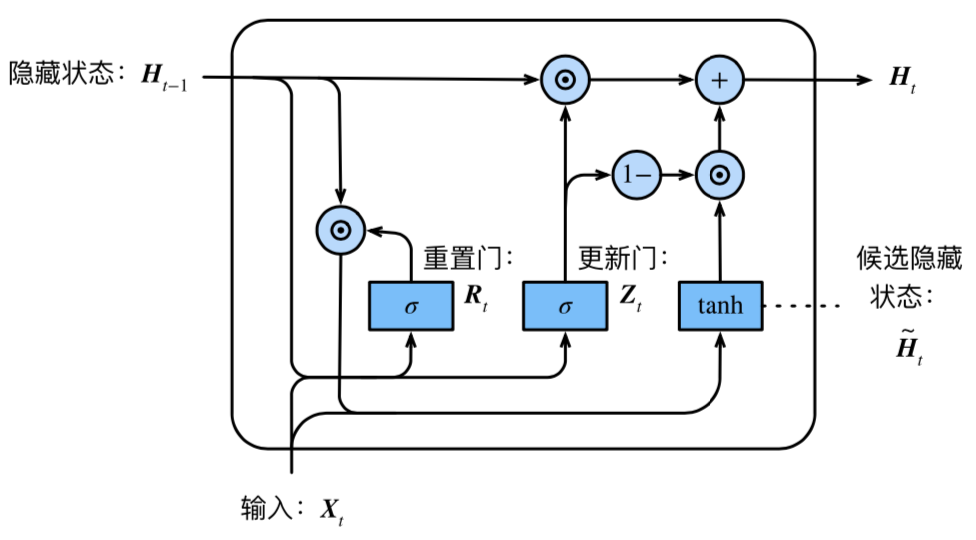
\includegraphics[width=0.6\textwidth]{note_images/GRU.png} %插入图片,[]中设置图片大小,{}中是图片文件名
  \end{figure}

  \textbf{reset gate重置门 update gate更新门}:

  \quad 得到上一层影藏层结果$H_{t-1}$ 当前时间步输入$X_t$

  \quad 重置门$R_t = \sigma(X_tW_{xr} + H_{t-1}W_{hr} + b_r)$
  
  \quad 更新门$Z_t = \sigma(X_tW_{xz} + H_{t-1}W_{hz} + b_z)$

  \quad \quad W 为权重参数\ b为偏差参数 $\sigma$为sigmoid函数

  \textbf{候选隐藏状态}

  \quad 候选隐藏状态$\tilde{H_t} = tanh(X_tW_{xh} + (R_t \odot  H_{t-1})W_{hh} + b_h)$

  \quad \quad $\odot$为按元素相乘,使得重置门中对应位置值为0的元素被丢弃

  \textbf{隐藏状态}

  \quad $H_t = Z_t \odot H_{t-1} + (1-Z_t)\odot \tilde{H_t}$
  
  输出公式不变:$O_t = H_tW_{hq} + b_q$\\
\textbf{LSTM长短期记忆} 门控循环网络
  \begin{figure}[H] %H为当前位置,!htb为忽略美学标准,htbp为浮动图形
    \centering %图片居中
    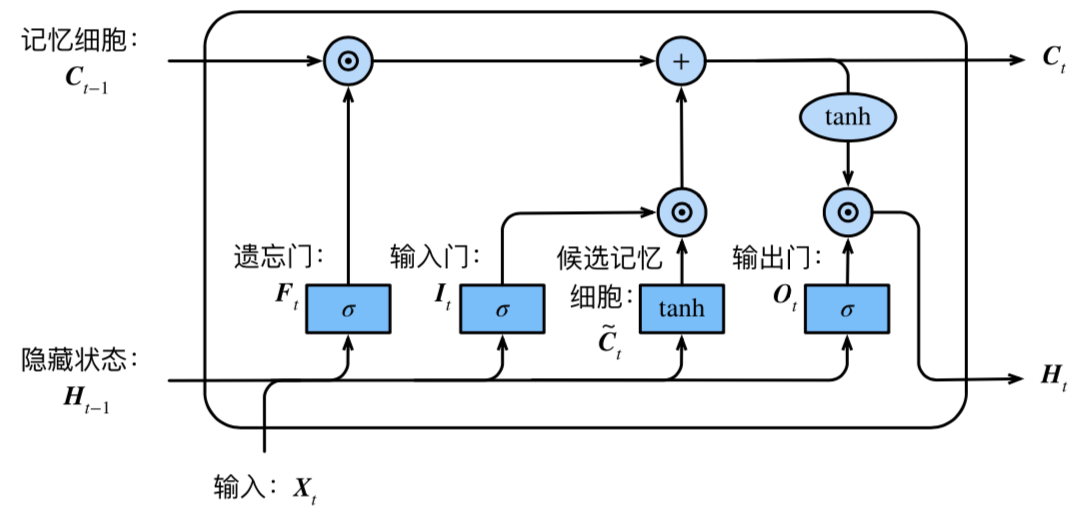
\includegraphics[width=0.6\textwidth]{note_images/LSTM.png} %插入图片,[]中设置图片大小,{}中是图片文件名
  \end{figure}
  
  \textbf{input gate输入门 forget gate遗忘门 output gate输出门 候选记忆细胞}

  \quad 输入门$I_t = \sigma(X_tW_{xi} + H_{t-1}W_{hi} + b_i)$

  \quad 遗忘门$F_t = \sigma(X_tW_{xf} + H_{t-1}W_{hf} + b_f)$
  
  \quad 输出门$O_t = \sigma(X_tW_{xo} + H_{t-1}W_{ho} + b_o)$

  \quad 候选记忆细胞$\tilde{C}_t = tanh(X_tW_{xc} + H_{t-1}W_{hc} + b_c) $

  \textbf{记忆细胞}

  \quad $C_t = F_t \odot C_{t-1} + I_t \odot \tilde{C}_t$

  \textbf{隐藏状态}

  \quad $H_t = O_t \odot tanh(C_t)$\\
\textbf{深度循环神经网络}

  包含多个隐藏层的RNN
  \begin{figure}[H] %H为当前位置,!htb为忽略美学标准,htbp为浮动图形
    \centering %图片居中
    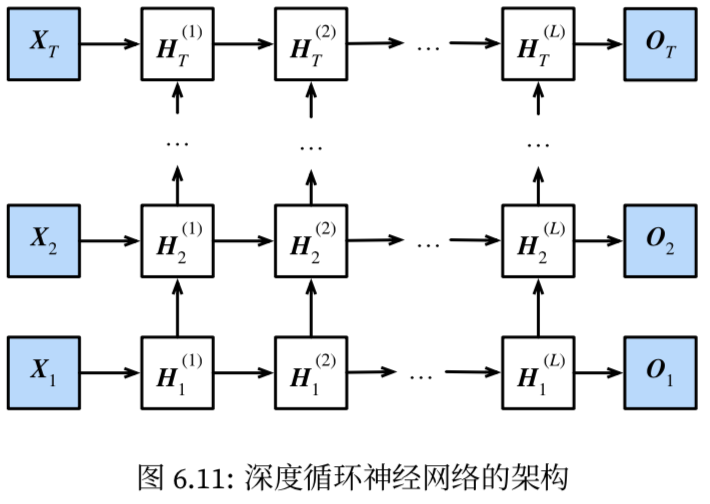
\includegraphics[width=0.6\textwidth]{note_images/deep_RNN.png} %插入图片,[]中设置图片大小,{}中是图片文件名
  \end{figure}
  结构:

  \quad 隐藏层\textbf{输出}为$H_i^{(1)} \space H_i^{(2)}...H_i^{(n)}$,第$i$次forward对应图中一行,即$X_i \rightarrow  H_i^{(1)} \rightarrow  ... \rightarrow  H_i^{(n)} \rightarrow O_i$

  \quad 第$i$次计算中:

  \quad \quad $l = 1$ 隐藏层输出 $H_i^{(1)} = \phi (X_iW_{xh}^{(1)} + H_{i-1}^{(l)}W_{hh}^{(1)} + b_h^{(1)})$

  \quad \quad \quad 和单层隐藏层RNN的\ 隐藏层输出公式\ 一致

  \quad \quad $l = 2,3...n$ 隐藏层输出 $H_i^{(l)} = \phi (H_i^{(l-1)}W_{xh}^{(l)} + H_{i-1}^{(l)}W_{hh}^{(l)} + b_h^{(l)})$

  \quad \quad \quad 即$l=1$公式中将输入变为前一隐藏层输出

  \quad \quad 输出层 $O_i = H_{i}^{(n)}W_{hq} + b_q$\\
\textbf{双向循环神经网络}

  允许神经网络根据前后的词序决定当前时间步的词
  \begin{figure}[H] %H为当前位置,!htb为忽略美学标准,htbp为浮动图形
    \centering %图片居中
    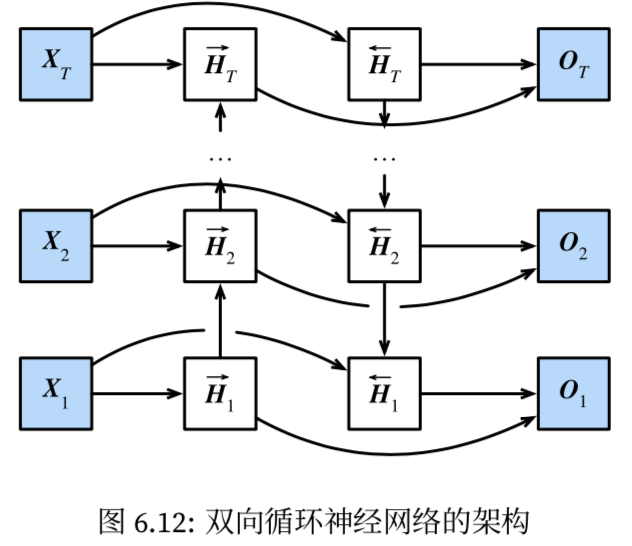
\includegraphics[width=0.6\textwidth]{note_images/double_deep_RNN.png} %插入图片,[]中设置图片大小,{}中是图片文件名
  \end{figure}
  结构:

  \quad 仅有2隐藏层,分为\ 正向隐藏层\ 反向隐藏层,分别输出$H^{(f)}$ $H^{(b)}$

  \quad 第$i$次计算中

  \quad \quad $H_i^{(f)} = \phi (X_iW_{xq}^{(f)} + H_{i-1}^{(f)}W_{hh}^{(f)} + b_h^{(f)})$

  \quad \quad $H_i^{(b)} = \phi (X_iW_{xq}^{(b)} + H_{i+1}^{(b)}W_{hh}^{(b)} + b_h^{(b)})$

  \quad \quad $O_i = H_iW_{hq} + b_q$

  \quad \quad \quad $H_i = (H_i^{(f)}, H_i^{(b)})$,为正向\ 反向隐藏层的输出concat\\
\textbf{经验总结}

  1. 增加一批量中的时间步数有助于提高周期性函数的预测效果

  2. ReLU做激活函数在周期性函数上预测效果较好


% --------------------------------------------------------------------------
% |                             代码算法优化                                 |
% --------------------------------------------------------------------------
\section{代码算法优化}
\noindent \textbf{Stochastic Gradient Decent 随机梯度下降}:采样方法

  每次迭代随机选择一个\textbf{样本},得到权重针对此样本的斜率进行梯度下降\ 而不是求参数针对所有样本的代价函数斜率。开销从O(n)变为O(1)

  \quad 即 任取的样本j,SGD迭代为$\theta_i = \theta_i - \eta \frac{d J^{(j)}(\theta)}{d \theta_i}$
  
  \quad 训练时noisy\\
\textbf{batch gradient descent 小批量随机梯度下降}:采样方法

  每次迭代随机选择一组样本 $B$,计算参数关于$B$的代价函数斜率

  \quad 分组目的为减少noisy,并避免需要迭代过整个训练集才能计算斜率

  重复采样:允许$B$中重复出现同一样本。反之不重复采样,

  随迭代次数增加,学习率可减小,使学习率和斜率的乘积方差减小\\
\textbf{动量法}:迭代方法

  解决固定一学习率值无法同时满足多个参数的学习率范围,导致某些参数发生学习太慢,某些参数不断越过最优解

  定义:
  
  \quad 向量$v_t$为第t次迭代每一参数的速度变量

  \quad 向量$x_t$为第t次迭代参数向量

  \quad 向量$g_t$为第t次迭代每一参数的斜率

  迭代:

  \quad $v_t = \gamma v_{t-1} + \eta_t g_t$

  \quad $x_t = x_{t-1} - v_t$\\
\textbf{adaptive learning rate}

  对每一参数使用不同learning rate,当参数更新较慢时增加学习率,反之减少
  
  以下迭代方法均为adaptive learning rate算法\\
\textbf{AdaGrad算法}:迭代方法

  根据参数斜率调整学习率

  定义向量$s_t$为第t次迭代累加变量,累计每一参数的斜率平方和

  迭代:

  \quad $s_t = s_{t-1} + g_t \odot g_t$

  \quad $x_t = x_{t-1} - \frac{\eta}{\sqrt{s_t + \epsilon } } \odot g_t$

  \quad \quad 即每一参数有变量记录所有斜率历史,每次迭代时\ 学习率/斜率历史l2 norm

  由于累加变量斜率历史,学习率始终降低,造成学习缓慢\\
\textbf{RMSProp 算法}:迭代方法

  解决AdaGrad末期学习率过低问题

  迭代:
  
  \quad $s_t = \gamma s_{t-1} + (1-\gamma)g_t \odot g_t$即 对$s_t$按元素平方做指数加权

  \quad $x_t$同AdaGrad算法\\
\textbf{AdaDelta 算法}:迭代方法

  解决AdaGrad末期学习率过低问题,不使用超参数

  定义:

  \quad 向量$g_t'$记录参数变化量

  \quad 向量$\varDelta x_t$对$g_t'$按平方做指数加权

  迭代:

  \quad $s_t = \gamma s_{t-1} + (1-\gamma)g_t \odot g_t$\ \ \ \ 同RMSProp

  \quad $\varDelta x_t = \gamma \varDelta x_{t-1} + (1-p)g_t' \odot g_t'$\ \ \ \ $\varDelta x_t$初始化为全零向量

  \quad $g_t' = \sqrt{\frac{\varDelta x_t + \epsilon }{s_t + \epsilon }} \odot g_t $

  \quad $x_t = x_{t-1} - g_t'$\ \ \ \ \ \ \ \ \ \ $g_t'$即参数变化率\\
\textbf{Adam 算法}:迭代方法

  定义:

  \quad $v_t$ t时间步的\ 动量变量

  \quad $s_t$ t时间步的\ 指数加权移动平均

  \quad $g_t$ t时间步\ 小批量\textbf{随机梯度}

  \quad $0\leq \beta_1<1$所有\ 动量变量的权重超参数。常取$0.9$
  
  \quad $1\leq \beta_2<1$ 所有\ 指数加权移动平均变量超参数。常取$0.999$

  迭代:

  \quad $v_t = \beta_1v_{t-1} + (1 -\beta_1)g_t$

  \quad $s_t = \beta_2 s_{t-1} + (1-\beta_2)g_t \odot g_t$

  \quad $\hat{v}_t = \frac{v_t}{1-\beta_1^t}$

  \quad $\hat{s}_t = \frac{s_t}{1-\beta_2^t}$

  \quad \quad 使用$\hat{v}_t$, $\hat{s}_t$\textbf{偏差修正}
  
  \quad \quad \quad 使得每一时间步t前的权重和为1,使得在时间步数较小时动量值不受权重影响

  \quad \quad \quad \quad 例:不使用偏差修正:$v_1 = 0.1g_1$

  \quad $g_t' = \frac{\eta \hat{v}_t}{\sqrt{\hat{s}^t} + \epsilon}$

  \quad \quad $\epsilon $常取$10^{-8}$

  \quad $x_t = x_{t-1} - g_t'$


% --------------------------------------------------------------------------
% |                              计算机视觉                                  |
% --------------------------------------------------------------------------
\section{计算机视觉}
\noindent 提升模型泛化能力方法:图像增广\ 图像微调\\
\textbf{图像增广}

  对图像随机变换,产生相似样本。扩大训练集

  方法:

  \quad 翻转:有固定几率上下/左右翻转

  \quad 裁剪:随机裁剪原图10\%-100\%面积的图像,宽高比0.5-2,并拉伸至固定像素大小

  \quad 变化颜色:调整亮度\ 色调\ 对比度\ 饱和度\\
\textbf{微调}

  假设:

  \quad 源模型包含的知识和目标模型紧密相连
  
  \quad 源模型输出层不能直接用于目标模型

  \quad 目标数据集远小于源数据集

  方法:
 
  \quad 1. 在源数据集上训练一神经网络,称源模型

  \quad 2. 创建一新神经网络,称目标模型,复制源模型除了输出层的所有结构和参数

  \quad 3. 为目标模型添加输出层,节点数对应输出种类,随机初始化模型参数

  \quad 4. 在目标数据集上训练目标模型,微调hidden layer参数,从头训练输出层参数

  \quad \quad 通过提高输出层学习率,降低隐藏层学习率达到重新训练输出层,微调隐藏层的目的。学习率相差可达1000倍\\
\textbf{目标检测\ 创建\ 匹配锚框算法}

  锚框:标记一个物体的范围框

  \quad 针对参数$s = {s_1, ..., s_n}$, $r = {r_1, ..., r_m}$

  \quad 为避免生成过多锚框,将图片分为不同区域grid,以每一区域中心生成锚框。区域grid可重叠

  \quad 每一grid生成$(s_1, r_1), (s_1, r_2), ..., (s_1, r_m), (s_2, r_1), ..., (s_n, r_m)$共$n+m-1$个锚框

  \quad 对$H, W$大小的图片,$h$行$w$列个区域情况中,每一区域中以$(s_i, r_j)$为参数的锚框有\ 高$ = s_i*\sqrt{r_j} * \frac{H}{h}$,宽$ = \frac{s_i}{\sqrt{r_j}} * \frac{W}{w}$

  \quad \quad \texttt{contrib.ndarray.MultiBoxPrior}和\texttt{d2l.torch.multibox\_prior}得到高$=\frac{s_i}{\sqrt{r_j}}$ 宽$ = s_i*\sqrt{a_j}$

  交并比IoU:两锚框\ 相交面积/相并面积

  训练集:每一锚框有对应的目标的标签\ 相对目标范围框的偏移

  \quad 赋目标框

  \quad \quad 1. 对锚框组$A_1, A_2, ...A_n$,目标框组$B_1, B_2, ...B_m$定义矩阵X,

  \quad \quad \quad X为(n, m),包含每一锚框相对每一目标框的交并比

  \quad \quad 2. 找到X中值最大项$x_{ij}$,则$A_i$对应目标$B_j$,移除X中$i$行$j$列

  \quad \quad 3. 重复找到剩余矩阵中的最大项并移除,最终有$m$锚框对应目标,剩余$n-m$锚框

  \quad \quad 4. 对每一未对应锚框$A_i$,寻找X中i行最大交并比,若值大于阈值,为$A_i$分配对应目标框,若没有交并比大于阈值,目标框为整个图片。

  \quad \quad 被赋予目标框的锚框称正类锚框,否则为负类锚框

  \quad 赋偏移量

  \quad \quad 对锚框$A_i$有坐标+长宽$(x_a, y_a, h_a, w_a)$,对应目标框$B_j$有$(x_b, y_b, h_b, w_b)$

  \quad \quad 设置常数$\mu_x = \mu_y = \mu_w = \mu_h = 0$, $\sigma_x = \sigma_y = 0.1$, $\sigma_w = \sigma_h = 0.2$

  \quad \quad 偏移量为$(\frac{\frac{x_b - x_a}{w_a} - \mu_x}{\sigma_x},\frac{\frac{y_b - y_a}{h_a} - \mu_y}{\sigma_y}, \frac{log(\frac{w_b}{w_a}) - \mu_w}{\sigma_w}, \frac{log(\frac{h_b}{h_a}) - \mu_h}{\sigma_h})$

  非极大值抑制:non-maximum suppression

  \quad 在显示结果阶段,去除重复对一个物体分类的锚框。\textbf{在训练结束后输出目标时使用,训练时直接使用所有锚框和标签集对比}

  \quad 锚框置信度:一个锚框$A_i$针对所有目标锚框$B$计算概率,$A_i$最大概率符合的目标锚框对应$A_i$的预测类别,此最大概率为$p$。概率不是锚框和目标锚框的交并比,而是输出层输出的\ 每一锚框与每一类别\ 的可能性

  \quad 算法:

  \quad \quad 1. 计算每一锚框置信度,选取最高的锚框$A_i$

  \quad \quad 2. 将所有和$A_i$交并比高于阈值的锚框删除

  \quad \quad 重复1.2.步,直至没有锚框剩余

  多尺度目标检测:仅适用部分像素点作为锚框的中心,减少锚框数量,减少计算\\
\textbf{SSD 单发多框检测}:一种目标检测算法

  \begin{figure}[H] %H为当前位置,!htb为忽略美学标准,htbp为浮动图形
    \centering %图片居中
    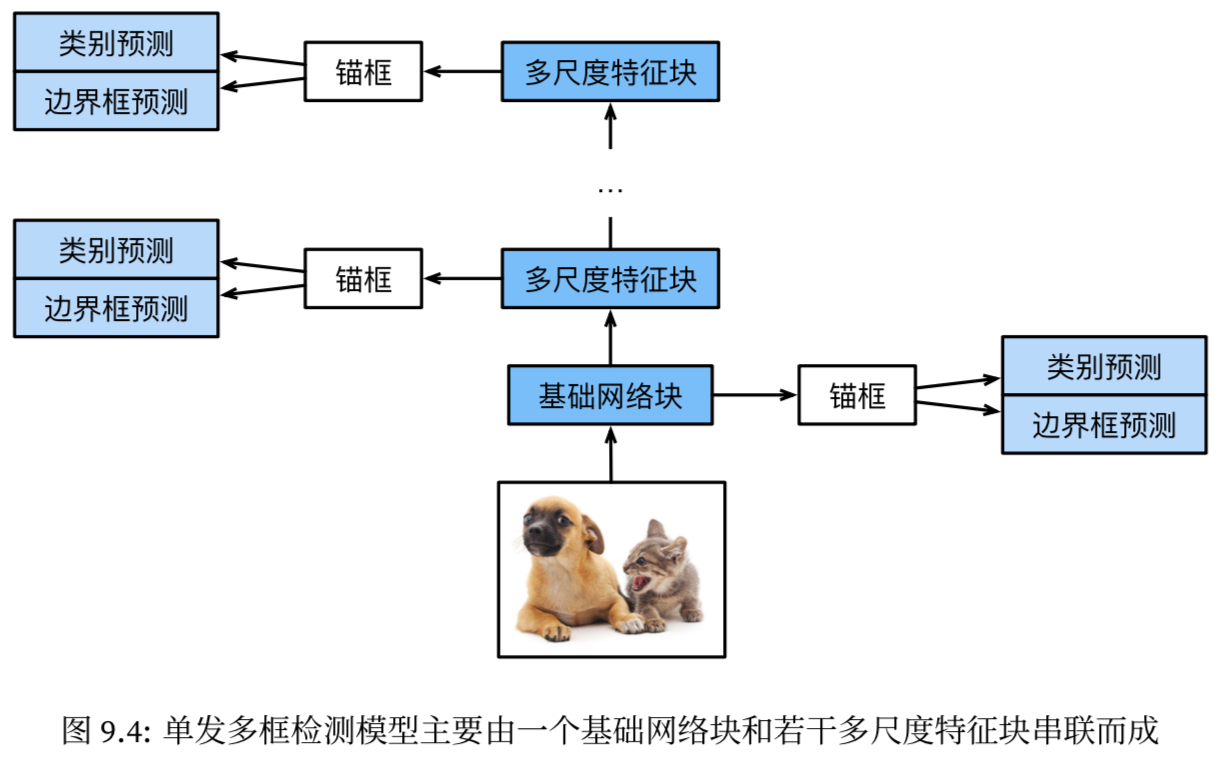
\includegraphics[width=0.6\textwidth]{note_images/SSD_archi.png} %插入图片,[]中设置图片大小,{}中是图片文件名
  \end{figure}

  \textbf{类别预测层}:

  \quad \textbf{得到卷积网络的张量,形状(批量大小,通道数,高,宽),处于同一高宽坐标的元素对应原图片中一区域grid 的像素,即原图区域为此元素的感受野。此区域中可包含多个锚框。}
    
  \quad 假设锚框中心像素有(h, w)个,每个中心点生成a个锚框,每个锚框需匹配进$(q+1)$个分类,多1分类对应负类分类

  \quad \quad 将锚框看做多层,每层$h*w$个,共$a$层,层编号为$c_1, c_2, ..., c_a$

  \quad 方法0:对每一锚框使用全连接层分类,即每一像素输入全连接网络,最终有匹配类别个数的输出层,判断锚框分类

  \quad \quad 造成参数过多,无法训练

  \quad 方法1:使用卷积层通道数输出类别

  \quad \quad 包含一个保持输入高\ 宽的卷积层,如\ 1填充 (3, 3)kernel的卷积层

  \quad \quad 输出通道数为$a * (q+1)$,每一通道输出仍为矩阵,第$(i-1)*(q+1) + j$通道包含锚框层$c_i$中所有锚框对分类j的匹配可能性。\textbf{由于输入张量每一元素对应一区域grid,卷积层输出(h, w)位置的值的可能性即为此锚框层属于(h, w)区域的锚框对一类别的预测可能性}

  \textbf{边界框预测层}:

  \quad 输入结构同类别预测层,输出通道数为$a * 4$,4对应一个锚框有4个偏差值,每一通道输出仍为矩阵,第$(i-1)*(q+1) + j$通道包含锚框层$c_i$中所有锚框的第$i$号偏差值

  \textbf{连接多尺度预测}:

  \quad 将不同多尺度特征块和基础网络块产生的\ 类别\ 边界预测层结果\ 合并
  
  \quad (批量大小, 通道数, 高, 宽)\ 转为 (批量大小, 通道数 * 高 * 宽)
  
  \textbf{高宽减半块}:

  \quad 1.两组[(3, 3)kernel 1填充\ 卷积层 + 批量归一化 + relu]
  
  \quad 2.(2, 2)窗口\ 2步幅\ 最大池化层

  \textbf{基础网络块}

  串联3块高宽减半块,分别有16, 32, 64通道

  \textbf{整体模型}
  
  \quad 结构对应图例,每一模块$l_i$对结果张量(批量大小, $h_i$, $w_i$)有\ 类别\ 边界预测层

  \quad 1. 基础网络块

  \quad 2-4. 高宽减半块,通道数都为128

  \quad 5. 仅包含全局最大池化层\ 高宽降至1

  \quad \textbf{得到输出集}

  \quad \quad 5层\ 类别\ 边界预测结果分别通过concat得到总体类别预测\ 边界预测,用于计算代价。

  \quad \quad \quad 类别分类concat结果:(批量大小,$\sum_i h_i * w_i$ * 锚框数,类别数+1)。

  \quad \quad \quad 边界预测concat结果:(批量大小,$\sum_i h_i * w_i$ * 锚框数 * 4),4对应偏移量个数
  
  \quad \quad 类别预测使用\texttt{SoftmaxCrossEntropyLoss},边界预测使用\texttt{L1Loss}。\textbf{由于所有坐标通过百分比表示,可直接和标签集一一对应,不受卷积层对矩阵大小影响}

  \quad \textbf{得到标签集}

  \quad \quad 对于5层中所有使用过的锚框,使用\textbf{目标检测}章节的算法对每一锚框添加标签\ 偏移量。
  
  \quad \quad 结果得到3个张量:
  
  \quad \quad \quad 每一锚框的类别,此张量所有元素和输出的类别预测进行交叉熵代价计算
  
  \quad \quad \quad 锚框数*4大小的bitmap,代表哪些锚框的偏移量被纳入代价函数计算。即\ 将此bitmap和第三张量按元素相乘\ 结果取平方和,为偏移量代价值
  
  \quad \quad \quad 锚框数*4大小的张量,代表每一锚框的偏移量。负类锚框的偏移量被忽略
  
  \quad \quad \quad \textbf{针对同一网络,不同迭代中产生的锚框位置\ 大小不变。由于目标框计算基于交并比,偏移量计算值不变。计算偏移量代价作用为:检查网络对偏移量的预估是否正确}\\
\textbf{R-CNN 区域卷积神经网络}

  对每一提议区域做卷积神经网络训练,耗时长\\
\textbf{Fast R-CNN}

  \begin{figure}[H] %H为当前位置,!htb为忽略美学标准,htbp为浮动图形
    \centering %图片居中
    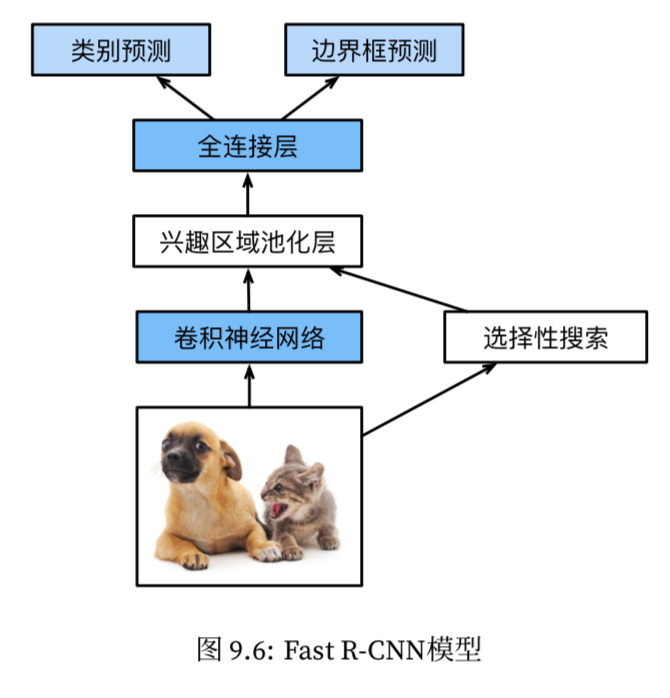
\includegraphics[width=0.6\textwidth]{note_images/Fast_R-CNN.png} %插入图片,[]中设置图片大小,{}中是图片文件名
  \end{figure}

  与\texttt{R-CNN}区别:

  \quad 1.提取特征的神经网络为整个图像

  \quad \quad 当输入为一张图片时,输出形状为$(1, c, h_1, w_1)$

  \quad 2.选择性搜索$n$个提议区域,

  \quad 3.兴趣区域池化层\ 输出$(n, c, h_2, w_2)$

  \quad \quad 可指定池化窗口任意矩形区域作为一个池化结果的源,所以可产生任意形状池化结果

  \quad \quad 例:
    $\begin{bmatrix}
      x_{11} & x_{12} & x_{13} \\
      x_{21} & x_{22} & x_{23} \\
      x_{31} & x_{32} & x_{33}
      \end{bmatrix}$
    可取$\begin{bmatrix}
      x_{11} & x_{12} \\
      x_{21} & x_{22} 
      \end{bmatrix}$
    和$\begin{bmatrix}
      x_{31} & x_{32}
      \end{bmatrix}$
    做输出$y_{11}$和$y_{21}$的来源

  \quad 4.全连接层\ 输出变为$(n, d)$,$d$为超参数

  \quad 5.预测类型使用$softmax回归$,输出$(n, q)$

  \quad \quad 预测边界框时,输出$(n, 4)$\\
\textbf{图像分割}

  区分图片中一个物体的不同部分,不将每一物体和标签对应\\
\textbf{实例分割}

  区分一个像素属于哪一物体,即使两物体为同一标签下的实例\\
\textbf{semantic segmentation语义分割}

  图像预处理:不使用拉伸,仅适用随机图片裁剪,裁剪得到图片一块固定形状的小图,作为训练集

  \textbf{FCN 全卷积网络}

  \quad 结构:
  
  \quad \quad 1.使用卷积神经网络\ 抽取图像特征

  \quad \quad 2.(1, 1)卷积层\ 通道数变为类别个数

  \quad \quad 3.转置卷积层\ 将图像的高宽变为输入图像的尺寸,作用仅为将2.中的图片分类反卷积得到图片表示,所以输入通道数 = 输出通道数 = 类别个数

  \quad 例:

  \quad \quad 1.ResNet-18预先训练神经网络抽取图像特征\ 丢弃最后全局平均池化层+全连接层

  \quad \quad 2.(1, 1)卷积层,通道数 = 类别数$n$
  
  \quad \quad 3.转置卷积层将(1, 1)卷积层每一通道的输出转换回图片大小的矩阵,每一元素为类别对应像素的index

  \quad 输出图片:
  
  \quad \quad 1.对一个图片的$n$个通道中结果\ 合并为唯一矩阵,新矩阵每一元素 = $n$个矩阵中对应位置最大值

  \quad \quad \quad 即\ 输出的$n$个矩阵代表图像符合每一类别的区域,对一个位置的元素取最大值即判断此位置最优先属于哪一类别
  
  \quad \quad 2.替换1.中输出的矩阵元素,每一元素替换为此位置的RGB向量\\
\textbf{样式迁移}

  \begin{figure}[H] %H为当前位置,!htb为忽略美学标准,htbp为浮动图形
    \centering %图片居中
    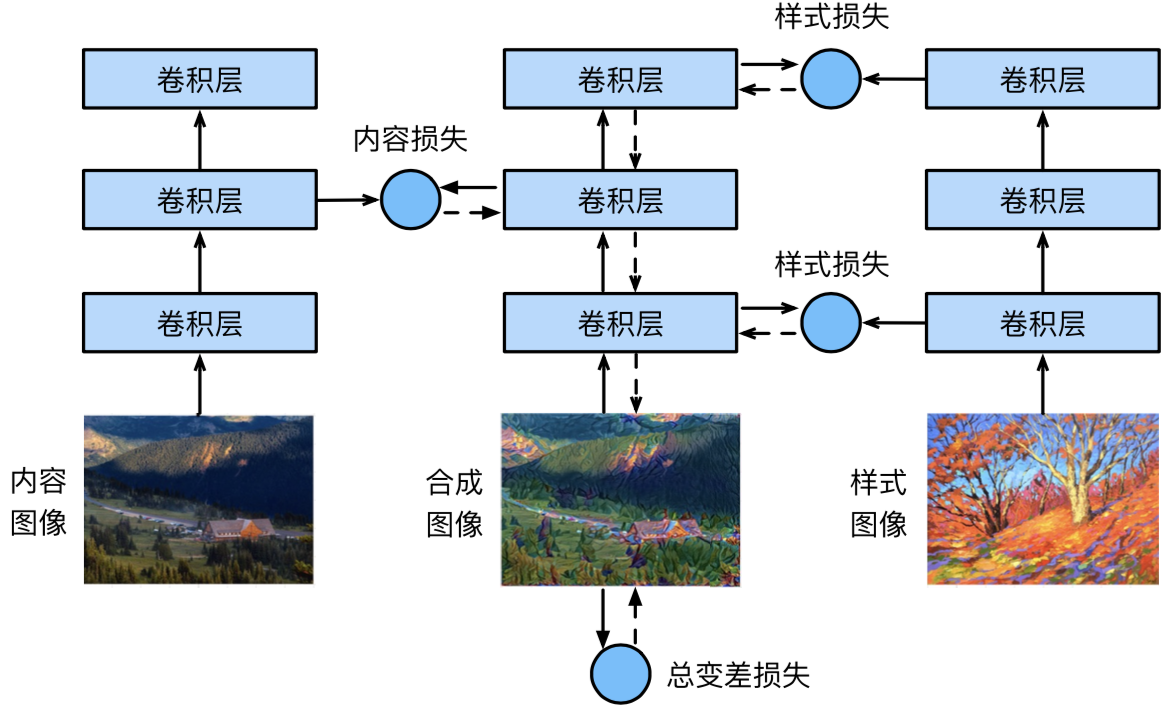
\includegraphics[width=0.6\textwidth]{note_images/style-transfer.png} %插入图片,[]中设置图片大小,{}中是图片文件名
  \end{figure}

  得到\ 内容图像\ 样式图像,输出合成图像

  \textbf{图像预处理}:将输入图片在RGB\ 3通道内分别做标准化

  \textbf{图像后处理}:将输出矩阵标准化的值\ 转回\ 像素值

  \textbf{抽取特征}:

  \quad 使用VGG-19预训练参数抽取图像特征

  \quad \quad 选择VGG靠近输出的层,称内容层,避免保留过多内容图像的细节

  \quad \quad 选择多个中间层的输出匹配样式,称样式层

  \textbf{损失函数}

  \quad 损失函数为内容\ 样式\ 总变差损失函数的加权和

  \quad \textbf{内容损失函数}:

  \quad \quad 使用平均平方代价函数,计算\ 合成图像\ 和\ 内容图像\ 在\ 内容特征上的误差

  \quad \quad 输入张量为\ 内容图像和合成图像\ 通过抽取特征后内容层的输出

  \quad \textbf{样式损失函数}:

  \quad \quad 输入张量为样式层输入

  \quad \quad 对每一样式层:

  \quad \quad \quad 1.将$c$通道$(h, w)$的样式层输出转为$(c, hw)$的矩阵$X$

  \quad \quad \quad 2.计算$X$的Gram matrix, $XX^T$。元素$(XX^T)_{ij}$即$x_i \cdot x_j$,代表通道i和j的相关性。可对Gram matrix每一元素先除以$|X|$元素值,避免样式损失值过高

  \quad \quad \quad 3.传入内容图像\ 合成图像,对每一样式层输出做平均平方代价函数,每层代价相加为总样式损失值

  \quad \textbf{总变差损失}:

  \quad \quad 输入仅为合成图像,对合成图像使用总变差降噪

  \quad \quad $J = \sum_{i, j} |x_{i,j} - x_{i+1,j}| + |x_{i,j} - x_{i,j+1}|$

  \quad \quad \quad 即\ 对每一合成图片的像素,求其和右方\ 下方像素的差值。最后求和

  \textbf{样式迁移模型}:

  \quad 使用每一VGG块的第一卷积层做样式层,第四卷积块的最后一卷积层做内容层
  
  \quad \textbf{更改的参数仅有生成的图片,不对网络参数进行更改}

% --------------------------------------------------------------------------
% |                             自然语言识别                                 |
% --------------------------------------------------------------------------
\section{自然语言识别}
\noindent \textbf{一. 词嵌入}

  词赋予两个向量$v_o, v_c$,分别为将词作为中心词和作为背景词使用的词向量
  
  \quad 词间夹角$\frac{u_o^Tv_c}{||u_o||\space||v_c||} \in [-1, 1]$为词的相似度

  定义:

  \quad $S$:词序集合,包含多个词序,包含重复的词

  \quad $\mathcal{V} $:所有词的索引集合,即$nub(S)$

  \quad $w_i$:一个词,索引为$i$

  \quad $v_i$:词$w_i$对应的实数向量
  
  \quad \quad 向量夹角余弦值$\frac{x^Ty}{||x||\space ||y||}$代表两个词的关联程度

  \quad 背景窗口大小$n$:定义对一个中心词$w_i$,背景词取值范围$=[$中心词$-n$, 中心词$+n]$。
  
  \quad \quad 范围为词序内位置关系,不是索引序号关系。背景词和中心词必须在同一词序内

  \quad \quad 当中心词一侧背景词个数$l<n$,填充$n-l$个无效词,随后由掩码舍弃不进入代价函数计算。

  给定中心词$w_c$,有单个背景词$w_o$的概率$P(w_o | w_c) = \frac{exp(u_o^Tv_c)}{\sum_{i\in\mathcal{V} } exp(u_i^Tv_c)}$
  
  \quad $ log(P(w_o | w_c)) = u_o^Tv_c - log(\sum_{i\in\mathcal{V} } exp(u_i^Tv_c))$\\
\textbf{跳字模型}:
  
  基于一个\textbf{中心词}生成才其周围的多个\textbf{背景词}

  \textbf{似然函数}:代表一段词序发生的可能性

  \quad 对中心词$w_c$,产生所有窗口内的背景词的概率为(假设背景词间$independent$)$P(c) = \prod_{c-n<j<c+n, j \neq c} P(w_j | w_c)$

  \quad (假设每一中心词产生背景词的可能性independent) 产生整个词序$S$的可能性:
  
  \quad \quad $P(S) = \prod_{0\leq c \leq |S|} P(c) = \prod_{c = 0}^{|S|-1} \prod_{j = c-n, j \neq c}^{c+n} P(w_j | w_c)$
  
  \textbf{代价函数}:基于似然函数,高似然代表低代价函数值

  \quad $J = -log(P(S)) = -\sum_{c = 0}^{|S|-1} \sum_{j = c-n, j \neq c}^{c+n} log(P(w_j | w_c))$
  
  \quad 求导: $\frac{d J}{d v_c} = -\sum_{c = 0}^{|S|-1} \sum_{j = c-n, j \neq c}^{c+n} \frac{d log(P(w_j | w_c))}{d v_c}$

  \quad \quad 对于每一中心词$v_c$有$\frac{d P(w_j | w_c)}{d v_c} = u_o^T - \sum_{j\in\mathcal{V}}P(w_j | w_c)u_j$\\
\textbf{连续词袋模型}

  与跳字模型不同处:中心词由背景词产生,和跳字模型相反

  给定背景词$W_o = w_{o_1}, w_{o_2}, ..., w_{o_{2m}}$,中心词$w_c$有出现概率:
  
  \quad $P(w_c | w_{o_1}, ..., w_{o_{2m}}) = \frac{exp(\frac{1}{2m}u_c^T(v_{o_1} + ... + v_{o_{2m}}))}{\sum_{i\in \mathcal{V} } exp(\frac{1}{2m}u_i^T(v_{o_1} + ... + v_{o_{2m}}))}$

  \quad \quad $= \frac{exp(u_c^T\bar{v}_o)}{\sum_{i\in \mathcal{V} } exp(u_i^T\bar{v}_o )}$

  \quad 1.使用\texttt{postierior estimate}计算得到,忽视$P(w_c)$项

  \quad 2.$\frac{1}{2m}$项为额外添加,使$\bar{v}_o = \frac{(v_{o_1} + ... + v_{o_{2m}})}{2m}$

  \quad 3.背景词使用背景向量$w_o$而非$w_c$
  
  \textbf{似然函数}:

  \quad $\prod_{c \in \mathcal{V} } P(w_c | W_o)$

  \textbf{代价函数}:基于似然函数,高似然代表低代价函数值

  \quad $J = -log(\prod_{c \in \mathcal{V} } P(w_c | W_o))$

  \quad \quad $= -\sum_{c \in \mathcal{V} } (u_c^T\bar{v}_o - log(\sum_{i\in \mathcal{V} } exp(u_i^T\bar{v}_o )))$

  \quad 求导:$\frac{d J}{d v_{o_i}} = -\frac{1}{2m}(u_c - \sum_{j \in \mathcal{V} }P(w_j | W_o)u_j)$\\
\textbf{近似训练}:对跳字模型和词袋模型的优化

  避免每次梯度计算都包含词典大小的项数计算

  \textbf{负采样}

  \quad 定义:

  \quad \quad 背景词$w_o$出现在$w_c$背景窗的概率为$P(D = 1|w_c, w_o) = \sigma(u_o^Tv_c)$

  \quad \quad \quad $\sigma$为sigmoid激活函数,$D = 1$代表事件发生,$D = 0$代表未发生

  \quad 更改$P(w_o | w_c)$定义:$P(w_o | w_c) = P(D = 1| w_c, w_o)\prod_{k=1, w_k \sim P(w)}^{K}P(D = 0 | w_c, w_k)$

  \quad \quad 根据$P(w)$分部取$K$个反样本,称噪声词,反样本不能为背景词

  \quad \quad \quad 根据word2vec论文,选择每一噪声词$w$的几率为$w$出现几率的0.75次方

  \quad \quad \textbf{加入反样本的原因:若最大化$P(D = 1|w_c, w_o) = \sigma(u_o^Tv_c)$,则所有词向量方向相同且长度极大}

  \quad 代价函数:$-log(P(w_o | w_c)) = -log(\sigma(u_o^Tv_c)) - \sum_{k=1, w_k \sim P(w)}^{K}log(1-\sigma(u_k^Tv_c))$

  \quad \quad $ = -log(\sigma(u_o^Tv_c)) - \sum_{k=1, w_k \sim P(w)}^{K}log(\sigma(-u_k^Tv_c))$
  \textbf{层序softmax}
  
  \quad 对整个词典有二叉树,每一分支节点$i$有背景词向量$u_i$,每一叶节点对应一词

  \quad 定义:

  \quad \quad $L(w)$:$w$在二叉树中的深度,包括根节点和叶节点

  \quad \quad $n(w, i)$:从根节点到$w$叶节点的路径上第j个节点,有背景词向量$u_{n(w, i)}$

  \quad \quad \quad \textbf{w在此为背景词,非中心词}

  \quad \quad \quad 一节点只有唯一背景词向量,当一节点出现在多个路径上时背景词向量被共享

  \quad 更改$P(w_o | w_c) = \prod_{j=1}^{L(w_o) - 1} \sigma(isLeftChild(n(w_o, j+1))) \cdot u_{n(w_o, j)}^Tv_c)$

  \quad \quad \begin{equation*}
    isLeftChild(x) = \begin{cases}
    1 &x < 0\\
    -1 & otherwise
    \end{cases}
  \end{equation*}

  \quad \quad 对固定中心词$w_c$,所有词的几率和为$\sum_{o \in \mathcal{V}} P(w_o | w_c) = 1$

  \quad \quad \quad 证明:选择任意节点$k$使得其左右子节点$i, j$都为叶节点

  \quad \quad \quad \quad $P(w_i | w_c) + P(w_j | w_c) = \prod ... \cdot (\sigma(x) + \sigma(-x))$

  \quad \quad \quad \quad $ = \prod ... \cdot 1$

  \quad \quad \quad \quad 即,任意仅有2页子节点的节点,子节点可能性和都为1。循环合并子节点,最终得到跟节点可能性为1\\
\textbf{二次采样}

  作用:对于一个词$w_0$,和低频词同时出现的情况\ 比\ 和高频词同时出现\ 对模型训练更加有用

  实现:
  
  \quad 取样的背景词中每个词有$P(w_i) = max(1-\sqrt{\frac{t}{f(w_i)}}, 0)$几率被丢弃

  \quad \quad $f(w_i) = $ 出现$w_i$个数 / 总词数,即词$w_i$在整个数据集中出现频率

  \quad \quad $t$为超参数

  \quad 对每个$w \in S$,使用二次采样随机丢弃$w$,创建新的$S'$作为训练集\\
\textbf{word2vec词嵌入模型实现}

  目标:\textbf{得到每一词的词向量,使有关联的词间向量夹角最小}

  \textbf{嵌入层}

  \quad 得到词嵌入的层,输入词$w_i$索引$i$,输出权重矩阵第$i$行作为词向量

  \quad 嵌入层有权重矩阵,形状\texttt{(词典大小, 每个词向量纬度)}

  \textbf{前向计算}

  \quad 输入:中心词索引矩阵
    $\begin{bmatrix}
      [c_1] \\
      ... \\
      [c_b]
      \end{bmatrix}
    $+ (背景词, 噪声词)索引矩阵
    $\begin{bmatrix}
      [o_{11}, ..., o_{1n}, q_{11}, ..., q_{1k}] \\
      ... \\
      [o_{b1}, ..., o_{bn}, q_{b1}, ..., q_{bk}]
      \end{bmatrix}
    $

  \quad \quad $b$为批量大小

  \quad \quad $n$为窗口大小

  \quad \quad $k$为噪声词数量

  \quad \quad 两个输入矩阵元素皆为常数,非向量

  \quad 1.通过嵌入层变换为\ 中心词向量张量\texttt{(b, 1, 词向量长)}
  $\begin{bmatrix}
    [u_{c_1}] \\
    ... \\
    [u_{c_b}]
    \end{bmatrix}
  $\ 背景噪声词向量张量\texttt{(b, n+k, 词向量长)}
  $\begin{bmatrix}
    [v_{o_{11}}, ..., v_{o_{1n}}, v_{q_{11}}, ..., v_{q_{1k}}] \\
    ... \\
    [v_{o_{b1}}, ..., v_{o_{bn}}, v_{q_{b1}}, ..., v_{q_{bk}}]
    \end{bmatrix}
  $

  \quad 2.对两张量小批量相乘,即得到\texttt{(b, 1, n+k)}张量
  $\begin{bmatrix}
    u_{c_1}^T [o_{11}, ..., o_{1n}, q_{11}, ..., q_{1k}] \\
    ... \\
    u_{c_b}^T [o_{b1}, ..., o_{bn}, q_{b1}, ..., q_{bk}]
    \end{bmatrix}
  $

  \quad 乘法为矩阵乘法,行向量$u_{c_1}^T$ 乘\ 矩阵$[o_{11}, ..., o_{1n}, q_{11}, ..., q_{1k}]$
  
  \quad 输出张量(b, 1, k+n),每一元素为背景词\ 噪声词和中心词的点乘,对应计算词向量夹角
  
  \textbf{代价函数}

  \quad 使用Sigmoid二元交叉熵函数,传入前向传播结果$P$,label$L$代表样本是否为正样本,掩码$M$代表样本是否有效

  \quad 目标为使预测结果$P$每一有效位置和$L$对应位置相同\\
\textbf{fastText子词嵌入}:基于word2vec优化

  产生子词:在单词首尾添加\texttt{< >},取所有长度为$s$的子字符串 + 单词本身

  \quad 如,对单词\texttt{'where'}有子词\texttt{\{'<wh', 'whe', 'her', 'ere', 're>', '<where>'\}}

  每一子词都存在词典中,单个词对应的向量为子词向量和\\
\textbf{GloVe全局向量的词嵌入}:基于word2vec优化

  对每一中心词$w_i$,合并所有$w_i$的背景词,称多重集$\mathcal{C}_i$。多重集直接合并原集合,不删除重复项

  \quad 一个背景词$w_j$在$\mathcal{C}_i$中的出现次数称\ 重数,记做$x_{ij}$

  \quad 定义$x_i = |\mathcal{C}_i|$,为多重集集合大小

  \textbf{代价函数 1}:$J = -\sum_{i\in \mathcal{V} }\sum_{j\in \mathcal{V} }x_{ij} \space log(P(x_j | x_i))$  

  \quad $= -\sum_{i\in \mathcal{V} }x_{i} \sum_{j\in \mathcal{V} } \frac{x_{ij}}{x_i}\space log(P(x_j | x_i))$

  \quad 第二层求和即\ 实际样本中$w_j$出现在$w_i$背景集合中的概率$\frac{x_{ij}}{x_i}$\ 和\ 模型预测的出现概率$P(x_j | x_i)$的交叉熵

  \quad * 较少使用,计算开销较大。并包含大量生僻词,导致预测准确率较低

  \textbf{代价函数 2}:使用平方代价函数$J = \sum_{i \in \mathcal{V}}\sum_{j \in \mathcal{V}}h(x_{ij})(u_j^Tv_i + b_i + c_j -log(x_{ij}))^2$

  \quad $h(x_{ij})$为权重,在$[0, 1]$单调递增

  \quad \quad 例:\begin{equation*}
    h(x) = \begin{cases}
    0 & x = 0\\
    (x / c)^{0.75} & x < c\\
    1 & x > c
    \end{cases}
  \end{equation*}

  \quad \quad c可取100

  \quad $b_i$为中心词偏差项,$c_j$为背景词偏差项

  \quad $u_j^Tv_i$即$x_{ij}$,$log(x_{ij})$即$P(x_j|x_i)$除去分子
  
  \textbf{GloVe每一词的背景词向量和中心词向量相同,由于每对词互为背景词。}最终每一词的背景词向量 = 中心词向量 = 所求的$u_c + u_o$
  
  \quad 预测$P(w_i | w_j)$公式不变
  
  \textbf{证明代价函数}
  
  \quad 针对词向量,定义函数$f(u_i, u_j, u_k)$使得对一个词$w_k$,其余两个词相对出现的几率$\frac{P(w_i | w_k)}{P(w_j | w_k)} \approx f(u_i, u_j, u_k)$
  
  \quad \quad 函数$f(u_i, u_j, u_k)$可定义为标量函数$g((u_i - u_j)^Tu_k)$
  
  \quad \quad $g(x)$需满足$g(x)g(-x) = 1$,则g可取$g(x) = exp(x)$
  
  \quad 则需要$\frac{exp(u_i^Tu_k)}{exp(u_j^Tu_k)} \approx \frac{P(w_i | w_k)}{P(w_j | w_k)}$

  \quad 则$P(w_i | w_k) = \frac{x_{ki}}{x_k} = \alpha \cdot exp(u_i^Tu_k)$

  \quad \quad $u_i^Tu_k = log(\alpha) + log(x_{ki}) - log(x_k)$

  \quad 中心词偏差项$b_k$和背景词偏差项$c_i$之和$b_k + c_i$模拟$-log(\alpha) + log(x_k)$

  \quad 则最小化$u_i^Tu_k + b_k + c_i - log(x_{ki})$,使用平方代价函数\\
\textbf{求近义词}:word2vec应用

  使用KNN,在训练结束的词向量中寻找余弦值最小的K个向量\\
\textbf{求类比词}:word2vec应用

  给定词$w_a, w_b, w_c$,求$w_d$使得$w_a : w_b$关系类似$w_c:w_d$

  算法:使用KNN,寻找向量临近$v_b - v_a + v_c$\\
\textbf{二. 文本情感分类}

  分析文本作者的情感

  输入:多组\ 词序\texttt{长度n} + 标记的情感类型

  \textbf{使用循环神经网络}:

  \quad 1.使用预先训练的嵌入层得到词向量

  \quad 2.双向循环神经网络

  \quad \quad 每一隐藏状态分别有形状(批量大小,2 * 隐藏单元个数),*2 由于为双向网络

  \quad 3.全连接层,得到分类的情感

  \quad \quad 输入为双向循环神经网络\ 第一和最后一隐藏状态\ 连接后的张量,有形状(批量大小,4 * 隐藏单元个数)

  \textbf{使用卷积神经网络textCNN}

  \quad 1.使用预先训练的嵌入层得到词向量,即输入形状为(词向量长度$d$,词数$L$)

  \quad 2.卷积计算:多个一维卷积核$k_i$,每一卷积核为\ (输出通道个数$c_i$, 词向量长度$d$,卷积核宽$w_i$)形状的矩阵

  \quad \quad 对一个卷积核一通道的计算,将每一卷积核窗口内的输入按元素相乘求和。输出形状(1, 词数 - 核宽 + 1)

  \quad \quad 总输出为一列表矩阵,有形状$[(c_0, L - w_0 + 1), (c_1, L - w_1 + 1), ...]$

  \quad \quad 同一维卷积核有唯一核宽长度相同,不同一维卷积核可使用不同核宽

  \quad 3.时序最大池化层:类似一维全局最大池化层
  
  \quad \quad 针对单一一维卷积核的输出$(c_i, L - w_i + 1)$,对$c_i$个输入通道各得出$L - w_i + 1$时序内最大值。即输出一向量,长度为$c_i$
  
  \quad 4.将所有时序最大池化层结果\texttt{concat}

  \quad 5.全连接层,将\texttt{concat结果分类为情感}\\
\textbf{seq2seq 编码器-解码器}

  对不定长输入$[x_1, ..., x_T]$允许输出为不定长序列$[y_1,...y_{T'}]$,使用定长的背景向量$c$做连接\ 解码器-编码器\ 的中间向量

  定义:输出词集合为$\mathcal{Y} $,其中包含一个$<eol>$特殊词代表词序末尾

  \textbf{编码器}:将不定长输入序列变为定长背景变量$c$

  \quad 对每一时间步$i$,字符$w_i$,使用循环神经网络隐藏层计算隐藏状态$h_i$。即输出$[h_0, ..., h_T]$

  \quad 长度为$T$序列$s_i$有背景向量$c = q(h_1, ..., h_T)$。q为自定义函数

  \textbf{解码器}:根据前一输出序列和$c$,输出结果序列

  \quad 根据解码器隐藏状态$s_{t'} = g(y_{t'-1}, c, s_{t'-1})$计算$P(y_i | y_{1}, .., y_{i-1}, c)$
  
  \quad 对一个序列的输出,总可能性为$ P(y_1,...,y_{T'} | x_1, ..., x_T)$。此值目标为此值最大化

  \textbf{代价函数}

  \quad $-log(P(y_1,...,y_{T'} | x_1, ..., x_T)) = -log(\prod_{i=1}^{T'} P(y_i | x_1, ..., x_T))$

  \quad \quad $ = -\sum_{i=1}^{T'}log(P(y_i | x_1, ..., x_T))$
  
  \textbf{解码器算法}:

  \quad \textbf{贪婪搜索}:每一$y_i = argmax_{y\in \mathcal{Y} }P(y|y_1, ..., y_{i-1})$

  \quad \quad 即每次取$y_i$使得$[1, i]$范围内$P$值最高,直至$i = T'$

  \quad \quad $y_{i-1}$对$y_i$的取值造成影响,若最优解$y_i$位置的词非第$i$时间步的$argmax$则贪婪算法无法取到最优解

  \textbf{beam search 束搜索}
  
  \quad 定义:beam size束宽$k$

  \quad 计算:
  
  \quad \quad 1.时间步$i = 1$,选取条件概率最大$k$个值,做$k$个可选序列的首词
  
  \quad \quad 2.时间步$i = 2,3...,L$,对每一可选输出序列考虑整个$\mathcal{Y} $,将$k*\mathcal{Y} $个新时间序列看做一整体,选出$P$值最高的$k$个作为此序列的下一词。最终每一时间步的输出序列都作为可选序列进入第三步,共$L*K$个时间序列。
  
  \quad \quad \quad 即,永远保持$k$个序列,而一个时间序列可能添加不同的$\hat{y}$而在下一时间步预测中有多个分支。
  
  \quad \quad 3.将$L*k$个序列筛选,仅保留包含$<eol>$的词序,舍弃$<eol>$后的词
  
  \quad \quad 4.在3.的序列集合中选择值$\frac{1}{l^a}log(P(y_1, ...,l))=\frac{1}{l^a}\sum_{i=1}^llog(P(y_i|y_1, ..., y_{i-1}, c))$最大序列作为输出
  
  \quad \quad \quad $l$为每一序列长度,$a$为参数,常取0.75。$\frac{1}{l^a}$惩罚长度较大项\\
\textbf{注意力机制}

  编码器对每一时间步产生背景向量$c_i'$而非对整个词序产生唯一背景向量$c$

  计算背景变量$c_{t'}$:

  \quad 计算每一编码器隐藏状态$h_t$的权重$\alpha_{t't} = \frac{exp(e_{t't})}{\sum_{t=1}^{T}exp(t't)}$,即对不同$t$的$e_{t't}$求softmax

  \quad \quad $e_{t't}$同时基于编码器时间步$t$和解码器时间步$t'$,则可定义$e_{t't} = a(s_{t'-1}, h_t)$。

  \quad \quad \quad a函数例:当$s_{t'-1}, h_t$长度相等,$a(s_{t'-1}, h_t) = s_{t'-1}^Th_t$

  \quad \quad \quad 注意力机制论文:$a(s_{t'-1}, h_t) = v^Ttanh(W_ss + W_hh)$,$v, W_s, W_h$为可学习参数

  \quad 对所有时间步内的编码器隐藏状态$h_t$求加权平均,即背景变量$c_{t'} = \sum_{t=1}^{T}\alpha_{t't}h_t$

  计算解码器隐藏状态:(类似GRU算法,加入背景变量项)
  
  \quad $s_{t'} = z_{t'} \odot s_{t'-1} + (1-z_{t'}) \odot \tilde{s}_{t'}g(y_{t'-1}, c_{t'}, s_{t'-1})$

  \quad \quad 重置门$r_{t'} = \sigma(W_{yr}y_{t'-1} + W_{sr}s_{t'-1} + W_{cr}c_{t'} + b_r)$
  
  \quad \quad 更新门$z_{t'} = \sigma(W_{yz}y_{t'-1} + W_{sz}s_{t'-1} + W_{cz}c_{t'} + b_z)$

  \quad \quad 候选隐藏状态$\tilde{s}_{t'} = tanh(W_{ys}y_{t'-1} + W_{ss}(s_{t'-1} \odot r_{t'}) + W_{cs}c_{t'} + b_s)$

% --------------------------------------------------------------------------
% |                              推荐算法                                   |
% --------------------------------------------------------------------------
\section{推荐算法}
\noindent \textbf{collaborative filter CF}

  分类:
  
  \quad memory-based CF:如nearest neighbour-based CF (包括user-based CF, item-based CF),
  
  \quad model-based CF:matrix factorization 
  
  \quad hybrid CF

  \quad pointwise approach:从implicit feedback 得到推荐

  \quad \quad 针对每一组(用户,产品)关系得到推荐

  \quad pairwise approach:从implicit feedback 得到推荐

  \quad \quad 对每一用户,比较任意2产品的推荐程度

  定义:

  \quad 用户集合$U$,产品集合$I$, 用户u评分过的产品$I_u^+$

  \quad interaction matrix $R \in \mathbb{R}^{m \times n}$:对m个用户n个产品,创建$m \times n$矩阵,元素$(i, j)$为用户$i$对$j$产品的评分

  \quad sparsity:1 - interaction matrix中非空项个数 / $(n \times m)$

  \quad seq-aware mode:分离测试集方法,将时间戳最近的数据留作测试集

  \quad 训练集$D = {(u, i, j) | \forall u \in U, i \in I_u^+, j \in I \setminus I_u^+}$


  \textbf{matrix factorization model}

  \quad 定义:

  \quad \quad 参数使用梯度下降学习,如SGD或Adam

  \quad \quad k:latent factor size。远小于m,n

  \quad \quad \quad 代表每一产品将有k个特征,用户对某一k元素向量的特征感兴趣

  \quad \quad $P \in \mathbb{R}^{m \times k}$:user latent matrix

  \quad \quad \quad 第i行代表用户i对最感兴趣的产品特征

  \quad \quad $Q \in \mathbb{R}^{n \times k}$:item latent matrix

  \quad \quad \quad 第i行代表产品i的特征

  \quad \quad $b_u$:用户u的bias。$b_i$:产品i的bias

  \quad \quad $\hat{R}_{ui} = PQ^T_{ui} + b_u + b_i$

  \quad 代价函数:$\sum_{(u, i)} ||R_{ui} - \hat{R_{ui}}||^2 + \lambda(||P||_F^2 + ||Q||_F^2 + b_u^2 + b_i^2)$

  \quad \quad 即,对$\hat{R}$使用平方代价函数,对$P, Q, b_u, b_i$使用L2 正则 

  \textbf{item based AutoRec}

  \quad 得到一个产品$i$的评价向量$R_{*i} \in \mathbb{R}^m$,每一元素为一用户对此产品的评价。
  
  \quad 输出一向量$\hat{R_{*i}} \in \mathbb{R}^m$,每一元素$R_{ji}$对应此产品对用户$j$的吸引力。

  \quad $\hat{R}_{*i} = f(W \cdot g(VR_{*i} + \mu) + b)$

  \quad \quad f, g为激活函数。可取f为linear activation,g为sigmoid + 0.05 dropout层

  \quad 代价函数:$\sum_{i=1}^{m}||R_{*i} - \hat{R_{*i}}||_O^2 + \lambda (||W||_F^2 + ||V||_F^2)$

  \quad \quad 即对每一用户,计算对其偏好向量的预测,和实际的偏好向量求平方代价函数。

  \quad \quad 此模型假设所有产品的数据使用同一转换得到实际用户对产品的需求。

  \textbf{Bayesian Personalized Ranking Loss BPRLoss}:一种pairwise ranking代价函数

  \quad 预测:对一用户$u$,在产品$i, j$中用户偏向产品$i$的可能性为:$p(u, i, j) = \sigma(\hat{y}_{ui} - \hat{y}_{uj})$。
  
  \quad \quad $\hat{y}$为前向计算得到的用户$u$对产品$i$的偏向程度

  \quad 目标:最大化posterior probability$p(\theta | >_u) \propto p(>_u | \theta)p(\theta)$

  \quad \quad $\theta$代表参数,$>_u$代表实际用户对产品的排名。

  \quad \quad 则最大化posterior estimate$ln(p(\theta | >_u)) \propto ln(\prod_{(u, i, j) \in D} \sigma(\hat{y}_{ui} - \hat{y}_{uj})p(\theta))$

  \quad \quad \quad $ = \sum_{(u, i, j) \in D} ln(\sigma(\hat{y}_{ui} - \hat{y}_{uj})) + ln(p(\theta))$

  \textbf{Hinge Loss}:一种pairwise ranking代价函数

  \quad $\sum_{(u, i, j) \in D} max(m - \hat{y}_{ui} + \hat{y}_{ij}, 0)$

  \quad \quad $m$为超参数

  \quad \quad 即:需要前向计算结果对两产品预测差值至少达到$m$,否则增加代价值

  \textbf{NeuMF}:一种neural CF

  \quad GMF部分:

  \quad \quad 针对user,item latent matrix $P \in \mathbb{R}^{m \times k}$,$Q \in \mathbb{R}^{n \times k}$

  \quad \quad $\hat{y}_{ui}^{MLP} = P_u \odot V_i$。即对$P, Q$的u行和i行按元素相乘
  
  \quad \quad 反向传播更新$P, Q$

  \quad MLP部分:

  \quad \quad 有$U \in \mathbb{R}^{m \times k}$,$V \in \mathbb{R}^{n \times k}$

  \quad \quad 连接$U_u$和$V_i$行,使用全连接神经网络,输出$\hat{y}_{ui}^{MLP}$

  \quad \quad 反向传播更新$U$,$V$,所有神经网络层参数

  \quad 前向传播

  \quad \quad 连接$[\hat{y}_{ui}^{GMF}, \hat{y}_{ui}^{MLP}]$。
  
  \quad \quad 使用单一全连接层,输出标量结果$\hat{y}_{ui} = f(h^T[\hat{y}_{ui}^{GMF}, \hat{y}_{ui}^{MLP}])$

  \quad 代价函数使用BPRLoss

  \quad ** 分析结果 **:

  \quad \quad hit rate at cut off $l$:$Hit @ l = \frac{1}{m}\sum_{u \in U}(rank_{} \leq l)$

  \quad \quad \quad 取用户$u$倾向的产品,求其中在推荐列表中排名前$l$名的个数。对所有用户重复操作,求个数和。

  \quad \quad AUC:ROC曲线下方的面积

  \quad \quad \quad $AUC = \frac{1}{m}\sum_{u \in U}\frac{1}{|I \setminus |}$
  
% --------------------------------------------------------------------------
% |                         Information Theory                             |
% --------------------------------------------------------------------------
\section{Information Theory}
\noindent \textbf{self information}

  对长度为n的二进制数组X,self information$I(X) = -log_2(n)$\\
\textbf{information定义}

  0. \textbf{针对一random variable}

  1. 两个random variable的总体information$\leq$ 分别得到两variable information后求和值。当两random variable independent,总体information = 两者information之和

  2. 越固定的random variable,information 值越接近0
\textbf{Shannon Entropy}

  \textbf{针对一分部}

  对random variable$X \sim P$,pdf为$p(X)$。
  
  Shannon entropy为expected information $H(X) = -E_{x \sim P}(log(p(x)))$

  \quad X离散时$H(X) = - \sum_{x} p(x)log(p(x))$

  \quad X连续时$H(X) = -\int_{x} p(x)log(p(x)) \,dx $
  
  \textbf{取-log原因}
  
  \quad 取$X_1, X_2 \sim P$,由$p(X_1, X_2) = p(X_1)p(X_2)$,$logp(X_1, X_2) = log(p(X_1))log(p(X_2))$。满足information第1条定义
  
  \quad 取负,由于当$p(x)$升高时希望information值降低

  \textbf{Entropy 性质}

  \quad 令$X \sim P$,pdf为$p(x)$。当使用新分部 $Q$,pdf $q(x)$,estimate $X$时:

  \quad \quad $H(X) = -E_{x \sim P}(log(x)) \leq -E_{x \sim P}(log(q(x)))$。

  \quad \quad 仅当$Q = P$时等式成立

  \quad 令$X \sim P$。当X均匀分部时entropy最大。

  \quad \quad $H(X) \leq log(\frac{1}{k})$,离散P中k为类别数,连续P中k为值域

  \quad \quad 即均匀分部时random variable 在不同类别/不同取值中的总体information最大化\\
\textbf{joind entropy}

  $H(X, Y) = -E_{(x, y) \sim P}(log(p_{X, Y}(x, y)))$

  X,Y为离散random variable,$H(X, Y) = -\sum_x\sum_yp_{X, Y}(x, y)log(p_{X, Y}(x, y))$

  X,Y为连续random variable,$H(X, Y) = -\int_{x, y} p_{X, Y}(x, y)log(p_{X, Y}(x, y)) \,dxdy$

  $H(X), H(Y) \leq H(X, Y) \leq H(X) + H(Y)$
  
  \quad 证:当X,Y完全dependent,则$H(X) = H(Y) = H(X, Y)$。当X,Y完全independent,则$H(x) + H(Y) = H(X, Y)$\\
\textbf{conditional entropy}

  $H(Y | X) = -E_{(x, y) \sim P}(log(p(y | x)))$

  X,Y离散:$H(Y | X) = \sum_x\sum_yp_{X, Y}(x, y)log(\frac{p_{X, Y}(x, y)}{p_X(x)})$

  theorem: $H(Y | X) = H(X, Y) - H(X)$\\
\textbf{mutual imformation}

  定义:$I(X, Y) = H(X, Y) - H(X | Y) - H(Y | X)$

  \quad '被X, Y共享的information。除去给定X或Y就能决定另一random variable的entropy'

  \quad $ = E_xE_y(p_{X, Y}(x, y)log(\frac{p_{X, Y}(x, y)}{p_X(x)p_Y(y)}))$

  \quad $ = H(X) - H(X | Y) = H(Y) - H(Y | X)$

  \quad $ = H(X) + H(Y) - H(X, Y)$

  性质:

  \quad 1.symmetric:$I(X, Y) = I(Y, X)$

  \quad 2.non-negative:$I(X, Y) \geq 0$

  \quad 3.$I(X, Y)$ iff X, Y independent

  \quad 4.与3.相反,$I(X, Y) = I(X) = I(Y)$ iff X,Y有bijection\\
\textbf{Pointwise mutual information}

  $pmi(x, y) = log(\frac{p_{X, Y}(x, y)}{p_X(x)p_Y(y)})$

  (x, y)和假设$X, Y$independent时的近似程度\\
\textbf{Kullback-Leibler Divergence/relative entropy}

  计算两分部之间的距离

  令$X \sim P$,有pdf$p(x)$。使用另一分部$Q$估计$P$,有pdf$q(x)$

  relative entropy $D_{KL}(P || Q) = E_{x \sim P}(log(\frac{p(x)}{q(x)}))$

  \quad 当$p(x) < q(x)$,$log(\frac{p(x)}{q(x)}))$为负值,绝对值较大
  
  \quad 当$p(x) > q(x)$,$log(\frac{p(x)}{q(x)}))$为正值,绝对值较大

  性质:

  \quad non-symmetric:$D_{KL}(P||Q) \neq D_{KL}(Q || P)$

  \quad non-negative: $D_{KL}(P||Q) \geq 0$只有$P = Q$时取0

  \quad 当存在x使得$p(x) > 0$,$q(x) = 0$。定义$D_{KL}(P||Q) = \infty$

  \quad $I(X, Y) = D_{KL}(P(X, Y) || P(X)P(Y))$

  \quad \quad $ = E_Y(D_{KL}(P(X | Y) || P(X)))$

  \quad \quad $ = E_X(D_{KL}(P(Y | X) || P(Y)))$

% --------------------------------------------------------------------------
% |                         图像处理 (CV 课程笔记)                           |
% --------------------------------------------------------------------------
\section{图像处理 (CV 课程笔记)}
\noindent CMOS:RGB sensor

  Bayer filter:将输入光过滤为仅有R/G/B强度的光线,每一像素被分配为R/G/B中一种颜色

  \quad 在(2, 2)形状区域内对角线为R像素,剩余2像素分别为RB

  \textbf{令一像素被分配颜色A,显示时一RGB除A外的颜色值取相邻像素的平均值}\\
聚焦公式:

  令f为凸透镜焦距,u为物距,v为相距。则$\frac{1}{f} = \frac{1}{u} + \frac{1}{v}$\\
quantisation:相机得到颜色值为连续值,存储时为离散值。连续值转离散值称quantisation\\
image filter:

  卷积操作,步幅1\ 填充(卷积核边长 / 2)。
  
  Average filter:卷积核内所有值相同,相加为1。

  Gaussian filter:令卷积核中心为(0, 0)

  \quad $h(i, j) = \frac{1}{2\pi\sigma^2}e^{-\frac{i^2+j^2}{2\sigma^2}}$

  \quad \quad $ = h_x(i) h_y(j)$

  \quad \quad $h_x(i) = \frac{1}{2\pi\sigma^2}e^{-\frac{i^2}{2\sigma^2}}$,$h_y(j)$同理
  
  High-pass filter:

  \quad identity卷积核:仅有中心值为1,其余值都为0

  \quad high-frequency部分:identity卷积核 - average filter

  \quad high-pass卷积核 = identity - high-frequency卷积核。即卷积核中心以外的值相等,为负。中心值 > 1

  median filter:对卷积核覆盖的像素取中位数输出\\
linear time-invarient filter:当输入移动一offset时输出移动相同offset,并输出值不变\\
edge detection

  离散值中求导:
  
  \quad forward difference:$f'(x) = f(x + 1) - f(x)$

  \quad backward difference:$f'(x) = f(x + 1) - f(x)$
  
  \quad central difference:$f'(x) = \frac{f(x + 1) - f(x - 1)}{2}$

  卷积核中求导:forward:$[1, -1, 0]$,backward:$[[0, 1, -1]]$,central:$[1, 0, -1]$

  Prewitt filter:

  \quad 竖直卷积核$h_v = \begin{bmatrix}
    1 & 0 & -1 \\
    1 & 0 & -1 \\
    1 & 0 & -1
    \end{bmatrix}$
    水平卷积核$h_h = \begin{bmatrix}
      1 & 1 & 1 \\
      0 & 0 & 0 \\
      -1 & -1 & -1
      \end{bmatrix}$

  Sobel filter:

  \quad 竖直卷积核$h_v = \begin{bmatrix}
    1 & 0 & -1 \\
    2 & 0 & -2 \\
    1 & 0 & -1
    \end{bmatrix}$
    水平卷积核$h_h = \begin{bmatrix}
      1 & 2 & 1 \\
      0 & 0 & 0 \\
      -1 & -2 & -1
      \end{bmatrix}$

  \textbf{Prewitt filter, Sobel filter 2卷积核分别计算图像在水平/竖直方向的斜率}

  \quad $g_h = f * h_h$每一像素水平方向斜率,$g_v = f * h_v$像素竖直方向斜率

  \quad $g = \sqrt{g_h^2 + g_v^2}$此像素总体斜率

  \quad $\theta = tan^{-1}(g_v, g_h)$每一像素仅有唯一角度值

  Canny edge detection:

  \quad 使边界输出1,非边界为0

  \quad 1. 使用Gaussian filter减少noise

  \quad 2. 使用Prewitt或Sobel计算像素斜率

  \quad 3. 每一像素进行非极大值抑制得到单一标量,代表其为边界的权重

  \quad \quad 非极大值抑制\textbf{(不同于SSD)}:

  \quad \quad \quad 将像素周围角度分为8个区间,每一区间中心为一临近像素

  \quad \quad \quad 选择2区间使得\ 此像素角度值穿过两区间

  \quad \quad \quad 当两区间对应的像素\ 总体斜率\ 都小于此像素总体斜率,则此像素有权重为总体斜率,否则权重为0

  \quad 4. 边界权重在high threshould以上的像素有像素值1,在low high threshould间的像素有值0.5。否则像素值为0

  \quad 5. 对所有值为0.5的像素,若临近8像素有值为1像素,则此像素值调为1

  \quad \quad 可根据更新后的临近像素值判断是否调整0.5为1\\
Hough transformation:

  将边界检测图像结果转换为边界的函数表达式,允许有多个边界表达式

  \quad slope intercept form:$y = mx + b$

  \quad \quad 求解:每一边界像素(p, q)对应$q = mp + b$对应一m-b函数表达式

  \quad \quad \quad 对所有m-b函数,每一函数上点分配一权重。函数有交点时权重叠加
  
  \quad \quad \quad 最终权重大于一threshould的(m, b)点为一边界。

  \quad double intercept form:$\frac{x}{a} + \frac{y}{b} = 1$。即椭圆

  \quad normal form:$x\cos(\theta) + y\sin(\theta) = \rho$

  \quad \quad 求解:同slope intercept,函数为$\theta$-$\rho$

  \quad 圆弧边界:

  \quad \quad 方法1:$(x - a)^2 + (y - b)^2 = r^2$

  \quad \quad 方法2:$x = a + r\cos(\theta), y = b + r\sin(\theta)$
  
  \quad \quad \quad 限定$r \in [r_{min}, r_{max}]$

  \quad \quad \quad 对每一可能的r值求$a = x - r\cos(\theta)$, $b = y - r\sin(\theta)$,$\theta$取像素(x, y)位置的角度

  \quad \quad \quad 对(a, b, r)位置的权重+1,最终选择一组(a, b, r)使得权重高于一threshould\\
Interest Point Detection 

  image matching:将两张图中像素对应,如图片连接。为一种interest point detection 

  Harris detector:

  \quad 对图片一区域W内的像素

  \quad 定义$E(u, v) = \sum_{(x, y) \in W} w(x, y)[I(x + u, y + v) - I(x, y)]^2$

  \quad \quad $I(x, y)$即(x, y)位置像素亮度

  \quad \quad u, v为在水平/竖直方向的移动距离。$I(x + u, y + v)$可在W外

  \quad \quad $w(x, y)$为window function,
  
  \quad \quad \quad idle function:(x, y)在W内时为1,否则为0。
  
  \quad \quad \quad Gaussian function:不论(x, y)是否在W内,根据(x, y)距离W中心的距离取Gaussian分部值
  
  \quad Taylor expansion:

  \quad \quad $I(x + u, y + v) = I(x, y) + uI_x(x, y) + vI_y(x, y)$

  \quad \quad \quad $I_x, I_y$为图像在x, y位置的斜率**即$g_x, g_y$**

  \quad \quad 带入得$E(u, v) = [u, v]\sum_{(x, y) \in W}w(x, y)
    \begin{bmatrix}
      I_x(x, y)^2 & I_x(x, y)I_y(x, y) \\
      I_x(x, y)I_y(x, y) & I_y(x, y)^2
      \end{bmatrix}
    \begin{bmatrix}
      u \\ 
      v
      \end{bmatrix}$

  \quad \quad 令$M = \sum_{(x, y) \in W}w(x, y)
    \begin{bmatrix}
      I_x(x, y)^2 & I_x(x, y)I_x(x, y) \\
      I_x(x, y)I_x(x, y) & I_y(x, y)^2
      \end{bmatrix}$

  \quad \quad 则$M$symmetric,有$M = P 
    \begin{bmatrix}
      \lambda_1 & 0 \\
      0 & \lambda_2
      \end{bmatrix} P^T$

  \quad \quad \quad 当$M$为全零矩阵/$\lambda_1,\lambda_2 \sim 0$时,**(u, v)或(x, y)**不在边界

  \quad \quad \quad 当$M_{00} >> M_{11}$/$\lambda_1 >> \lambda_2$,在竖直edge上

  \quad \quad \quad 当$M_{00} << M_{11}$/$\lambda_1 << \lambda_2$,在水平edge上

  \quad \quad \quad 当$M_{00}, M_{11}$较大/$\lambda_1, \lambda_2$较大时,在边界拐点

  \quad 定义一点在拐点几率:

  \quad \quad Harris and Stephens:$R = \lambda_1\lambda_2 - k(\lambda_1 + \lambda_2)^2$,k常取0.05

  \quad \quad Kanade and Tomasi:$R = min(\lambda_1, \lambda_2)$

  \quad \quad Noble:$R = \frac{\lambda_1\lambda_2}{\lambda_1 + \lambda_2 + \epsilon}$

  \quad \quad 简化以上计算:$det(M) = \lambda_1\lambda_2$,$trace(M) = \lambda_1 + \lambda_2$

  scaling 后图像进行interest point detection:

  \quad Theorem:对函数$f(x)$,$g(sx) = f(x)$,有$\frac{df(x)}{dx} = s\frac{dg(sx)}{dx}$

  \quad $M = \sum_{(x, y) \in W}w(x, y)\sigma^2
    \begin{bmatrix}
      I_x(x, y, \sigma)^2 & I_x(x, y, \sigma)I_y(x, y, \sigma) \\
      I_x(x, y, \sigma)I_y(x, y, \sigma) & I_y(x, y, \sigma)^2
      \end{bmatrix}$

  \quad \quad 其中$I_x(x, y, \sigma)$为图像在(x, y)位置\ 放大$\sigma$\ 在水平方向的斜率

  Laplacian of Gaussian LoG:

  \quad 在使用Gaussian filter后求二阶导

  \quad \quad 求二阶导即对亮度$I$使用Laplace operator $\Delta I$,或使用卷积核$
    \begin{bmatrix}
      0 & 1 & 0 \\
      1 & -4 & 1 \\
      0 & 1 & 0
      \end{bmatrix}$

  \quad 合并Gaussian filter和求导操作:$\Delta (f * g) = f * \Delta g$,
  
  \quad \quad $f$为输入图像,$g$为二维Gaussian 卷积函数

  \quad \quad $ = f * (-\frac{1}{\pi\sigma^4}(1 - \frac{x^2 + y^2}{2\sigma^2})e^{-\frac{x^2 + y^2}{2\sigma^2}})$

  \quad **$LoG_{norm}(x, y, \sigma) = \sigma^2(I_{xx}(x, y, \sigma) + I_{yy}(x, y, \sigma))$**

  Difference of Gaussian DoG
  
  \quad $DoG(x, y, \sigma) = I * g(k\sigma) - I * G(\sigma)$
  
  \quad \quad $g(\sigma)$为使用$\sigma$的二维Gaussian卷积函数
  
  \quad **$DoG(x, y, \sigma) \approx (k - 1)\sigma^2\bigtriangledown^2G(x, y, \sigma)$**\\
Feature Description

  根据descriptor将不同图像上的像素对应

  \quad pixel intensity:相同intensity的像素一一对应

  \quad patch intensity:使一区域以内的像素intensity对应

  \quad gradient orientation:相同斜率和角度的像素对应

  \quad histogram:收集一区域以内的像素intensity 分部,相同分部的区域对应

  Scale-invariant Feature Transform SIFT

  \quad 目标:将图像转换为interest point,每一点有feature vector

  \quad 计算N个Gaussian filter结果,其中$\sigma$值取$\sqrt{2}, 2, 2\sqrt{2}, 4,...$

  \quad 相邻Gaussian filter间计算差值,得到N-1个DoG结果

  \quad key point assignment:**得到最优的$v = (x, y, \sigma)$使得$DoG(v)$最大化

  \quad \quad 通过Taylor 展开:$DoG(v + \delta) = DoG(v) + \frac{dDoG^T}{dv}\delta + \frac{1}{2}\delta^T\frac{d^2DoG}{dv^2}\delta$

  \quad \quad \quad 则$\frac{dDoG(v + \delta)}{d\delta} = \frac{dDoG}{dv} + \frac{d^2DoG}{dv^2}$

  \quad \quad \quad 取$\frac{dDoG(v + \delta)}{d\delta} = 0$,则$\delta = -\frac{d^2DoG}{dv^2}^{-1}\frac{dDoG}{v}$。$DoG(v + \delta)$有最值

  \quad orientation assignment:

  \quad \quad 在keypoint周围采样像素,窗口大小$\propto \sigma$

  \quad \quad 将采样的像素分入网格:每一网格内将方向分为8区间,采样的方向在8区域的分部

  \quad keypoint matching

  \quad \quad 使用euclidian distance对应两图key point

  \quad \quad 一对key point(u, v)(x, y)得到key point间转换表达式:

  \quad \quad \quad $[u, v]^T = 
    \begin{bmatrix}
      m_1 & m_2 \\
      m_3 & m_4
      \end{bmatrix}
    [x, y]^T + [b_1, b_2]^T$

  \quad \quad \quad 对所有key point pair$(u_i, v_i)$, $(x_i, y_i)$:

  \quad \quad \quad $
    \begin{bmatrix}
      x_1 & y_1 & 0 & 0 & 1 & 0 \\
      0 & 0 & x_1 & y_1 & 0 & 1 \\
      x_2 & y_2 & 0 & 0 & 1 & 0 \\
      0 & 0 & x_2 & y_2 & 0 & 1 \\
      ... 
      \end{bmatrix}
    \begin{bmatrix}
      m_1 \\
      m_2 \\
      m_3 \\ 
      m_4 \\
      b_1 \\
      b_2
      \end{bmatrix}
    =
    \begin{bmatrix}
      u_1 \\
      v_1 \\
      u_2 \\ 
      v_2 \\
      ...
      \end{bmatrix}$

  \quad \quad \quad 简写为Am = b
  \quad \quad \quad 求解$m = (A^TA)^{-1}A^Tb$
  
  Speeded-Up Robust Feature SRUF:feature descriptor

  \quad Haar wavelets:每一采样仅在水平/竖直方向取斜率$d_h, d_v$,斜率使用1/-1表示。(而非使用8方向的斜率求和)

  \quad descriptor:$(\sum d_x, \sum d_y, \sum |d_x|, \sum |d_y|)$

  Binary Robust Independent Elementary Feature BRIEF:

  \quad \begin{equation*}
      \tau(p, q) = \begin{cases}
      1 & h(p) > h(q)\\
      0 & otherwise
      \end{cases}
    \end{equation*}

  \quad 在一像素周围取$n_d$对像素$(p_i, q_i)$,descriptor为$\sum_{i \leq n_d} \tau(p_i, q_i) << i$

  \quad descriptor间距离为两descriptor XOR值\\
Histogram of Oriented Gradient HOG 

  对一区域的像素计算feature:

  \quad 将图像整体分为网格(非在某一像素周围分网格),每一grid计算gradient orientation histogram向量$v$

  \quad 多个grid 组成一block,有合并的locally normalized descriptor$v_{norm} = \frac{[v_1, v_2, ...]}{\sqrt{||[v_1, v_2, ...]||_2^2 + \epsilon^2}}$

  \quad 将block位置按卷积操作移动,HOG descriptor为所有block的descriptor连接\\
Optic Flow

  估计视频中的亮度在x,y方向分别移动(u, v)

  假设:

  \quad brightness constancy:两帧间物体上同一点亮度相同

  \quad small motion:两帧间物体上同一点移动距离较小

  \quad spatial coherence:相邻像素的移动方向相近
  
  由假设得$I(x + u, y + v, t + 1) = I(x, y, t) \approx I(x, y, t) + \frac{dI}{dx}u + \frac{dI}{dy}v + \frac{dI}{dt}$

  \quad 则对每一像素(x, y)都有$I_xu + I_yv + I_t = 0$

  Lucas-Kanade Method:计算(u, v)

  \quad 对每一像素$p_i$:$[I_x(p_i), I_y(p_i)][u, v]^T = [-I_t(p_i)]$

  \quad 令
    $A = 
    \begin{bmatrix}
      I_x(p_1) & I_y(p_1) \\ 
      I_x(p_2) & I_y(p_2) \\ 
      ...
      \end{bmatrix}$, 
    $x = [u, v]^T$,
    $b = 
    \begin{bmatrix}
      I_t(p_1) \\ 
      I_t(p_2) \\ 
      ...
      \end{bmatrix}$
    则Ax = -b

  \quad 取$x = argmin_x\|Ax + b\|$为最优$[u, v]^T$

  \quad 则有$x = (A^TA)^{-1}A^Tb$

  \quad \quad $A^TA = \sum_{p_i}
    \begin{bmatrix}
      I_x(p_i)^2 & I_x(p_i)I_y(p_i) \\ 
      I_x(p_i)I_y(p_i) & I_y(p_i)^2
      \end{bmatrix}$

  \quad \quad $A^Tb = - \sum_{p_i}
    \begin{bmatrix}
      I_x(p_i)I_t(p_i) \\ 
      I_y(p_i)I_t(p_i)
      \end{bmatrix}$

  Horn-Schunck method:每一像素有(u, v)

  \quad 最小化$E = \int_{p_i} (I_x(p_i)u + I_y(p_i)v + I_t(p_i))^2 + \alpha (\Delta u^2 + \Delta v^2) \,dxdy $

  \quad \quad 即最小化临近像素的方向向量改变量

  \quad 由Euler Lagrange equation:

  \quad \quad $(I_x(p_i)u + I_y(p_i)v + I_t(p_i))I_x(p_i) - \alpha\Delta u = 0$
  
  \quad \quad $(I_x(p_i)u + I_y(p_i)v + I_t(p_i))I_y(p_i) - \alpha\Delta v = 0$
 
  \quad \quad \quad $\Delta$为Laplace operator

  \quad 带入$\Delta u = \bar{u} - u$

  \quad \quad $(I_x(p_i)^2 + \alpha)u + I_x(p_i)I_y(p_i)v = \alpha \bar{u} - I_x(p_i))I_t(p_i)$
  
  \quad \quad $(I_y(p_i)^2 + \alpha)v + I_x(p_i)I_y(p_i)u = \alpha \bar{v} - I_y(p_i))I_t(p_i)$

  \quad 得到$u, v$关于$\bar{u}, \bar{v}$的公式

  Lucas-Kanade Tracker

  \quad 针对原图像I,J

  \quad 取(u, v),使得将图像I按(u, v)方向移动后和J像素平方差之和最小

  \quad \quad 即$\min_{u, v}\sum_{(x, y) \in pixels}(I(x, y) - J(x + u, y + v))^2$

  \quad 求解:对u, v微分

  \quad \quad $\frac{dE}{du} = 2\sum_{(x, y)}(I(x, y) - J(x + u, y  + v))\frac{d-J(x + u)}{du}$

  \quad \quad \quad $ = -2\sum_{(x, y)}(I(x, y) - J(x + u, y  + v))\frac{J}{dx}$

  \quad \quad \quad $ = -2\sum_{(x, y)}(I(x, y) - J(x, y) - \frac{dJ}{dx}u - \frac{dJ}{dy}v)\frac{J}{dx}$

  \quad \quad \quad $ = -2\sum_{(x, y)}(-I_t - I_xu - I_yv)I_x$

  \quad \quad \quad v公式同理:$ = -2\sum_{(x, y)}(-I_t - I_xu - I_yv)I_y$

  \quad \quad 令两微分值为0:

  \quad \quad \quad $-\sum_{(x, y)}
    \begin{bmatrix}
      I_xI_t \\
      I_yI_t
      \end{bmatrix} - \sum_{(x, y)}
    \begin{bmatrix}
      I_x^2 & I_xI_y \\
      I_xI_y & I_y^2
      \end{bmatrix}
    \begin{bmatrix}
      u \\
      v
      \end{bmatrix}
    = 0$

  \quad \quad \quad $
    \begin{bmatrix}
      u \\
      v
      \end{bmatrix}
    = 
    \sum_{(x, y)}
    \begin{bmatrix}
      I_x^2 & I_xI_y \\
      I_xI_y & I_y^2
      \end{bmatrix}^{-1}
    \sum_{(x, y)}
    \begin{bmatrix}
      I_xI_t \\
      I_yI_t
      \end{bmatrix}$\\
Camera Model 

  由2d图像预测观测点位置

  令$X = 
    \begin{bmatrix}
      x \\
      y \\
      z \\
      1
      \end{bmatrix}$, $
    \begin{bmatrix}
      x \\
      y \\
      z
      \end{bmatrix} 
    =
    \begin{bmatrix}
      p_1^T \\
      p_2^T \\
      p_3^T
      \end{bmatrix}
    \begin{bmatrix}
      x \\
      y \\
      z \\
      1
      \end{bmatrix}$

  prospective 投影后$x = \frac{p_1^TX}{p_3^TX}$, $y = \frac{p_2^TX}{p_3^TX}$

  \quad 可得$X^Tp_1 - X^Tp_3x = 0$, $X^Tp_2 - X^Tp_3y = 0$

  \quad $
    \begin{bmatrix}
      X^T & 0 & -X^Tx \\
      0 & X^T & -X^Ty
      \end{bmatrix}
    \begin{bmatrix}
      p_1 \\
      p_2 \\
      p_3
      \end{bmatrix}
    = 0$

  \quad \quad 令第一矩阵为A,有形状为(2, 12)。第二矩阵$\vec{p}$形状(12, 1)

  \quad 以上针对一像素(x, y, z)位置。对n个像素,第一矩阵形状为(2*n, 12),解$\vec{p} = argmin_p \|A\vec{p}\|^2$

  \quad \quad 加入条件$\|\vec{p}\| = 1$,使$\vec{p} = 0$不为有效解

  \quad \quad 求解:求SVD:$A = USV^T$,$\vec{p}$为A$V$中对对应最小singular value的列


% --------------------------------------------------------------------------
% |                       Deep Learning 第6章笔记                           |
% --------------------------------------------------------------------------
\section{Deep Feedforward Network (Deep Learning 第6章笔记)}
\noindent \textbf{SVM支持向量机}

  仍通过$w^Tx+b$得到输出,输出仅表示identity,正值说明有identity,负值说明没有

  依据:一个平面的公式为$\beta_0+\beta_1x_1+\beta_2x_2=0$,则当计算$w^Tx+b$得到值后,>0则为平面上方的数据点,<0为下方数据点\\
\textbf{kernel trick}

  kernel method将数据集表示成相近的两个数据点一组的集合$(x_i, x_j)$,kernel method将一对数据变为单一数据点$x=k(x_i, x_j)=\langle \phi (x_i), \phi (x_j)\rangle $

  kernel method使用$\phi $转换数据的纬度,而点乘 化简后无需先计算$\phi (x_i), \phi (x_j)$即可得到新数据点$x$\\
\textbf{manifold hypothesis:}

  当训练数据集合包含大量无规律的数据,则将其中大部分视为无效数据,并只关心落在一个manifold上的数据。

  例:生成图像 文字 声音时数据大多很集中,当像素文字随机分布时生成图像大多无意义\\
\textbf{deep feedforward network/feedforward neural network/multilayer perceptrons MLP:}

  找到$\theta$使得$f(x; \theta )$ 最接近数据y值。$f^*$为最理想的f,即$f^*(x) = y$。$\theta $可为多个参数,如$f(x; w, b) = x^Tw+b$

  $f^*(x) = f^{(3)}(f^{(2)}(f^{(1)}(x)))$,$f^{(1)}$为network第一层。每一$f^{(i)}(x) = \phi (x; \theta )^Tw$

  \textbf{神经网络}

  \quad 1. 结构:

  \quad \quad 输入层没有weight,第一hidden layer得到所有输入层的值。

  \quad \quad hidden layer和输出层所有输出都为0/1,非连续的值

  \quad 2. 一层hidden layer计算方法:$ f^{(i)}(x; W, c) = \sigma (W^Tx + c)$

  \quad \quad x 为前一层的输出向量,输入层x即为训练参数向量。 

  \quad \quad c 为此层常数向量

  \quad \quad z = $W^Tx$为一层hidden layer对输入取得的中间值向量,称logit。a = $\sigma (z + c)$为对z + c每一元素取$\sigma $的结果向量,a即此层的输出。

  \quad \quad W 为此层参数矩阵,行数 = 前层节点数,列数 = 当前层节点数

  \quad \quad X 为多个参数点的训练集中前一层的输出矩阵,行数为数据点个数,列数为前一层节点数

  \quad \quad $XW$ 当W对参数集矩阵操作时,每行向量$z_{i}^T$此时为一层hidden layer各节点对第i参数点的中间值向量。对每行+$c^T$并分别取$\sigma $得到输出矩阵,$a_{ij}$为当使用第i个参数点时此层第j节点的输出

  \textbf{cross entropy}

  \quad 分部p 和 分部q 间的 cross entropy $H(p, q) = -E_p(\log (q))$。为 expected value of $log (q)$ with respect to distribution p

  \textbf{cost function}

  \quad 当使用maximum likelihood估计参数时,cost function$J(\theta )$为 训练输入参数的分部 和 训练结果参数的分部 间cross-entropy: $J(\theta ) = -E_{x, y\sim training\_dataset}(log (p_{model}(y | x)))$

  \quad \quad 对于每一在训练集内的(x, y),求$log (p_{model}(y | x))$, 并求expected value。$p_{model}(y | x)$ 即训练得到的y关于x的分部

  \quad \quad 例:当model为$y = N(f(x; \theta), 1)$正则分部时,$J(\theta) = -E_{x, y\sim data}(y - f(x;\theta))^2 + const$

  \textbf{output layer}

  \quad 当输出层的结果和不为1时,代表数据没有被准确分到某一类中,使用exponentiation and normalisation

  \quad \quad normalisation后结果 $p = \frac{\tilde{p} }{\sum \tilde{p'} } $,为$\tilde{p} $在所有结果中占的比例。$\tilde{p} $为未normalise 值

  \quad 假设输出层结果$\tilde{P} (y | x)$ 有 $log(\tilde{P} (y | x)) = yz$

  \quad \quad $\tilde{P} (y | x) = exp(yz)$

  \quad \quad $P (y | x) = \frac{exp(yz)}{\sum_{y' = 0}^{1} y'z } $,称\textbf{softmax function}

  \quad \quad $P (y | x) = \sigma ((2y - 1)z)$,y,y'为训练目标结果,所以$\sum_{y' = 0}^{1} $包含所有y'

  \quad 对softmax function使用log likelihood原因:log $softmax(z)_i = z_i - log\sum_j exp(z_j)$。

  \quad \quad 当$z_i$为dominant,并对应期望的输出项。log $softmax(z)_i$ = 0。则此项不产生高cost,否则产生cost。

  \textbf{hidden unit}

  \quad \quad 代表一个hidden layer节点的激发函数。

  \quad \quad 1. rectified linear unit: $g(x) = max(0, x)$

  \quad \quad \quad 无法用于gradient based learning,由于一阶导为0

  \quad \quad \quad 基于rectified linear unit的优化:$g(x) = max(0, x) + a*min(0, x)$

  \quad \quad \quad \quad a = -1:absolute value rectifier

  \quad \quad \quad \quad a 为极小值:leaky ReLU

  \quad \quad \quad \quad a 为可学习值:Parametric ReLU, PReLU

  \quad \quad 2. Maxout units

  \quad \quad \quad 将x分为多组,每组h(x) 为组内最高值

  \textbf{backward propagation}

  \quad 一种计算gradient的方法,区别于使用gradient进行学习的stochastic gradient descent

  \quad 算法:
  \begin{figure}[H] %H为当前位置,!htb为忽略美学标准,htbp为浮动图形
    \centering %图片居中
    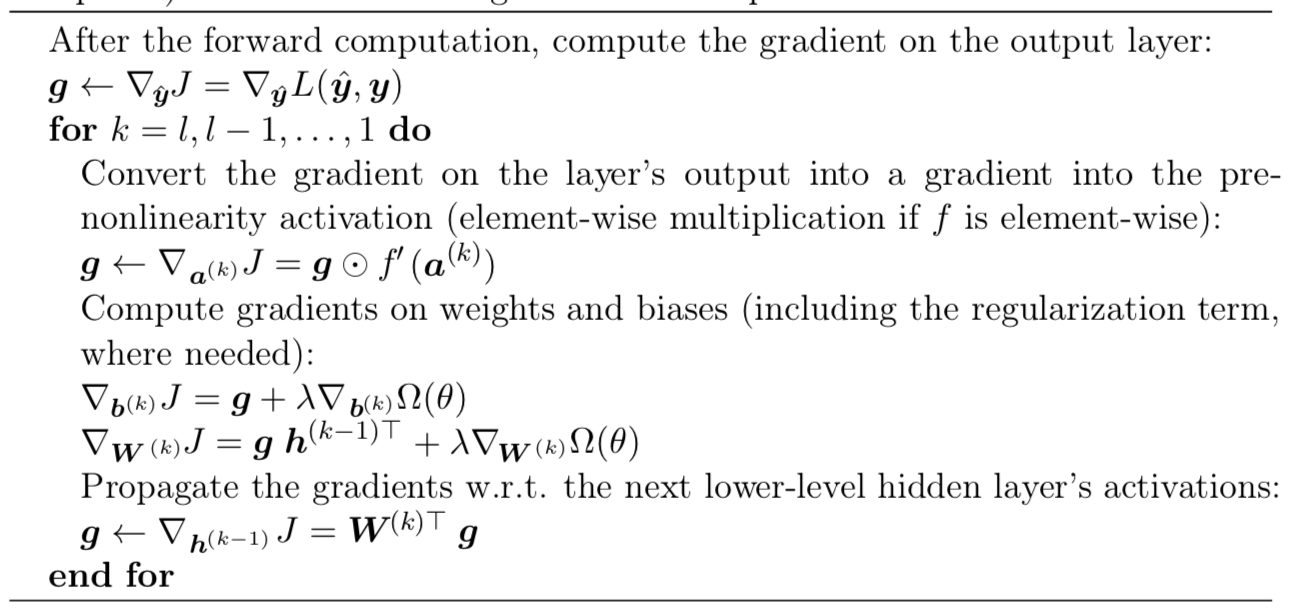
\includegraphics[width=0.6\textwidth]{note_images/backprop_algo.png} %插入图片,[]中设置图片大小,{}中是图片文件名
  \end{figure}

  
\end{document}
